En este anexo se presentan los resultados de las pruebas de accesibilidad realizadas en las vistas principales de la aplicación. 
Las capturas se han realizado con un iPhone 12 utilizando el navegador Safari en modo claro. Las especificaciones de la pantalla del dispositivo pueden consultarse
en \coloredUnderline{\href{https://support.apple.com/es-es/111876}{Apple - iPhone 12 - Especificaciones}}.

Se ha decido realizar las capturas de pantalla de las vistas principales de la aplicación en modo claro, ya que es el modo por defecto en el que se visualiza la aplicación. 
Además, solo se detallan las capturas para el iPhone 12, ya que es el dispositivo con la pantalla más pequeña y el que, por tanto, puede presentar más problemas de adaptabilidad.

\subsection*{Home}
\begin{figure}[H]
    \centering
    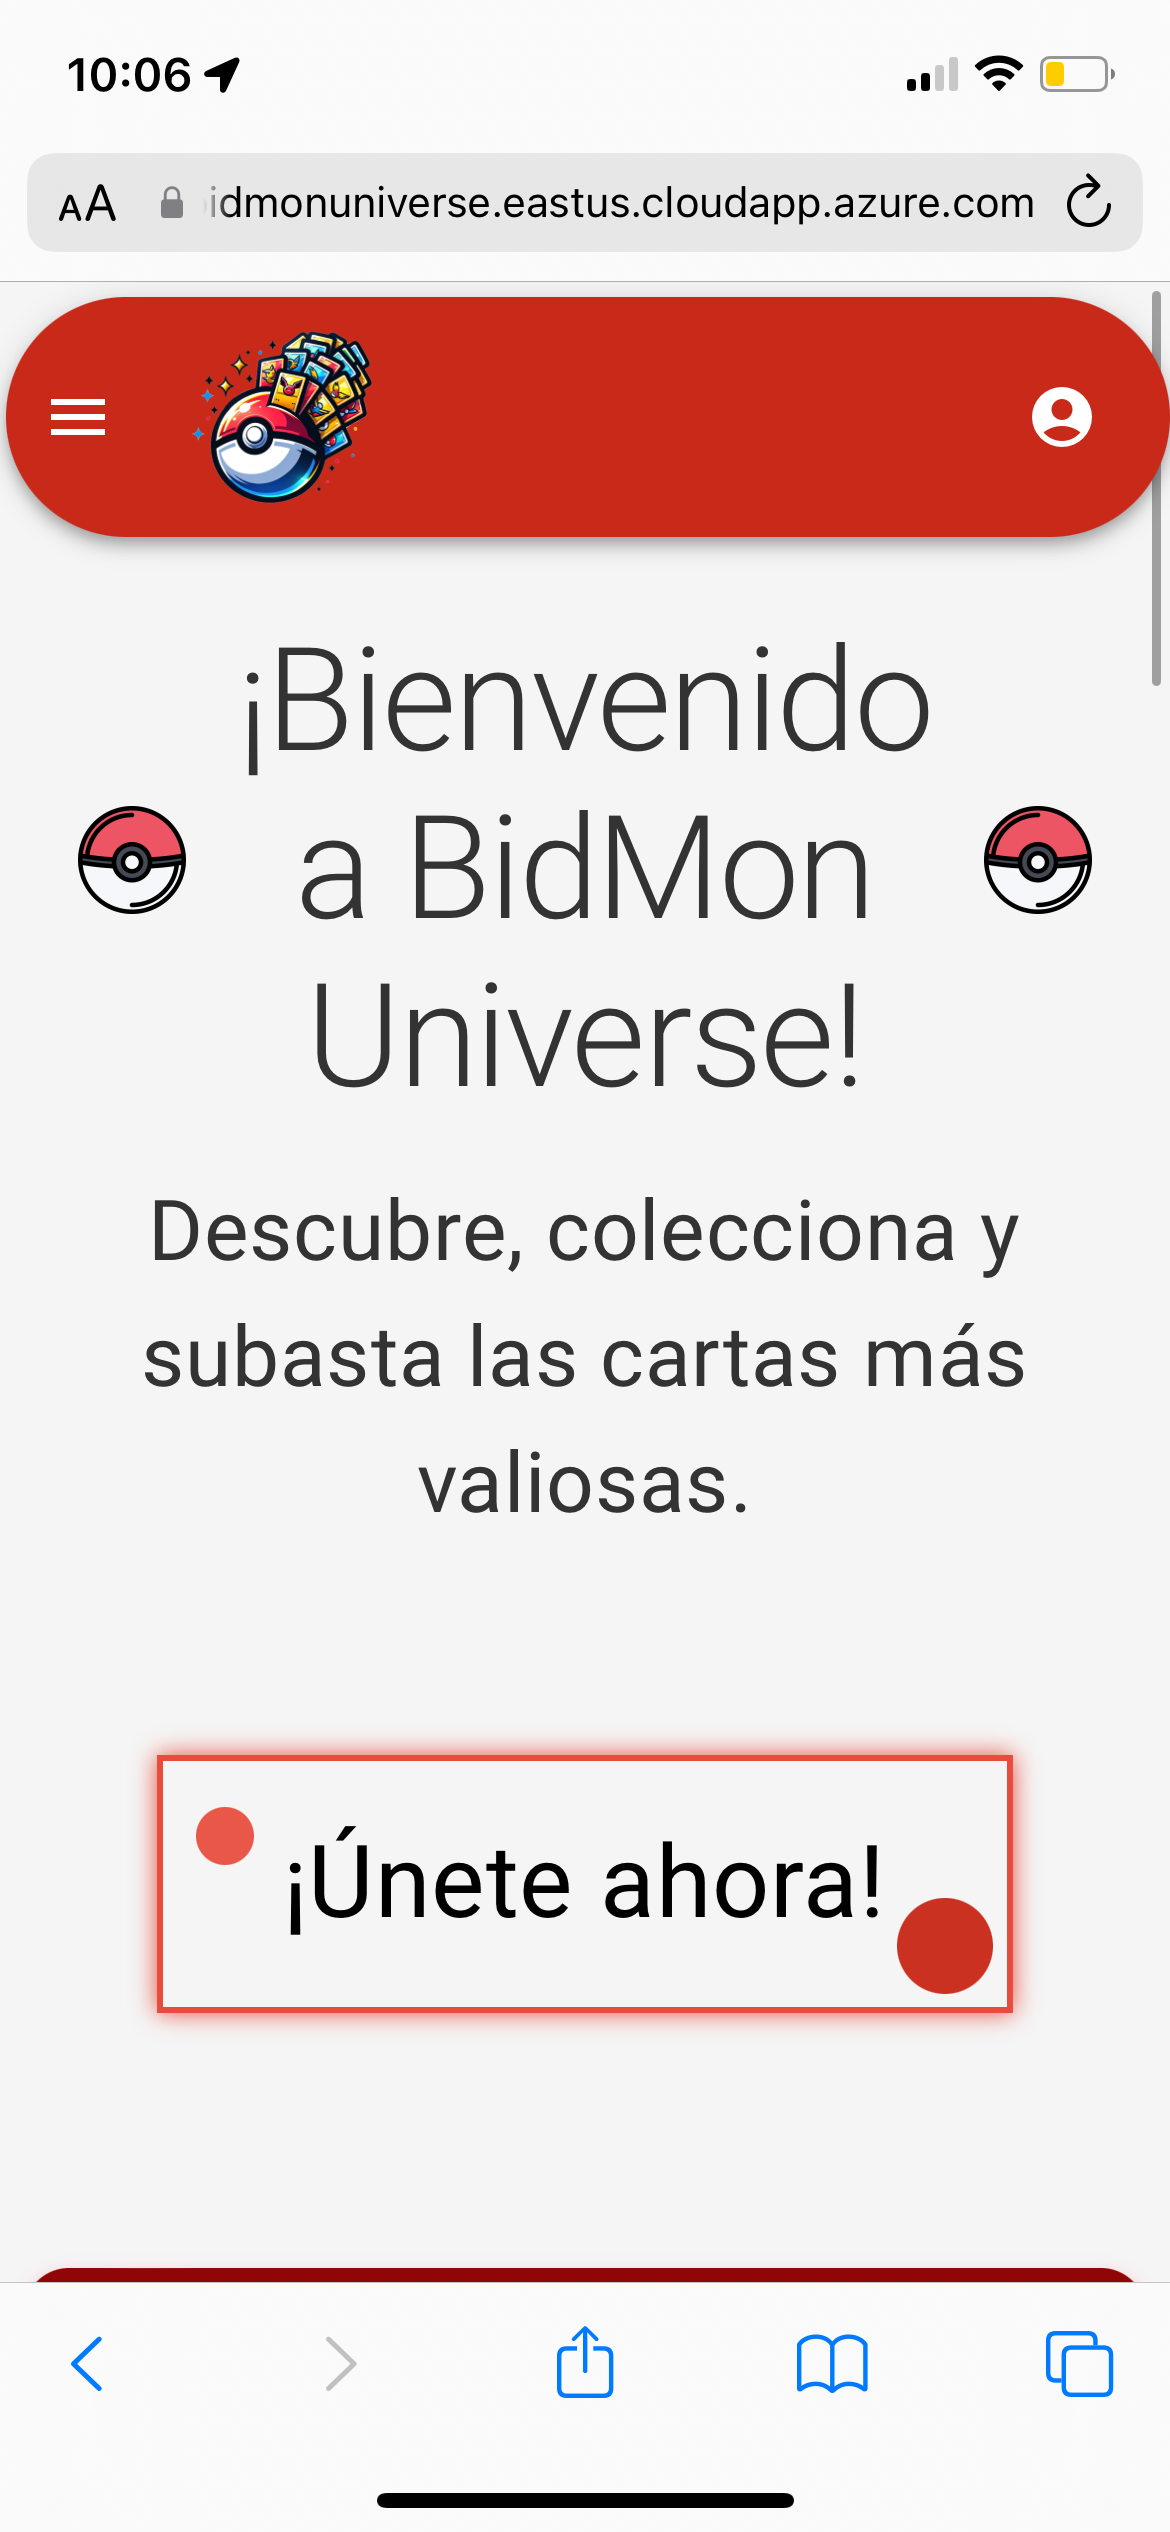
\includegraphics[ width=0.2\textwidth]{figures/adaptabilidad/home.png}
    \caption{Adaptabilidad Página Home}
    \label{fig:Adap-Home}
\end{figure}

\subsection*{Login}
\begin{figure}[H]
    \centering
    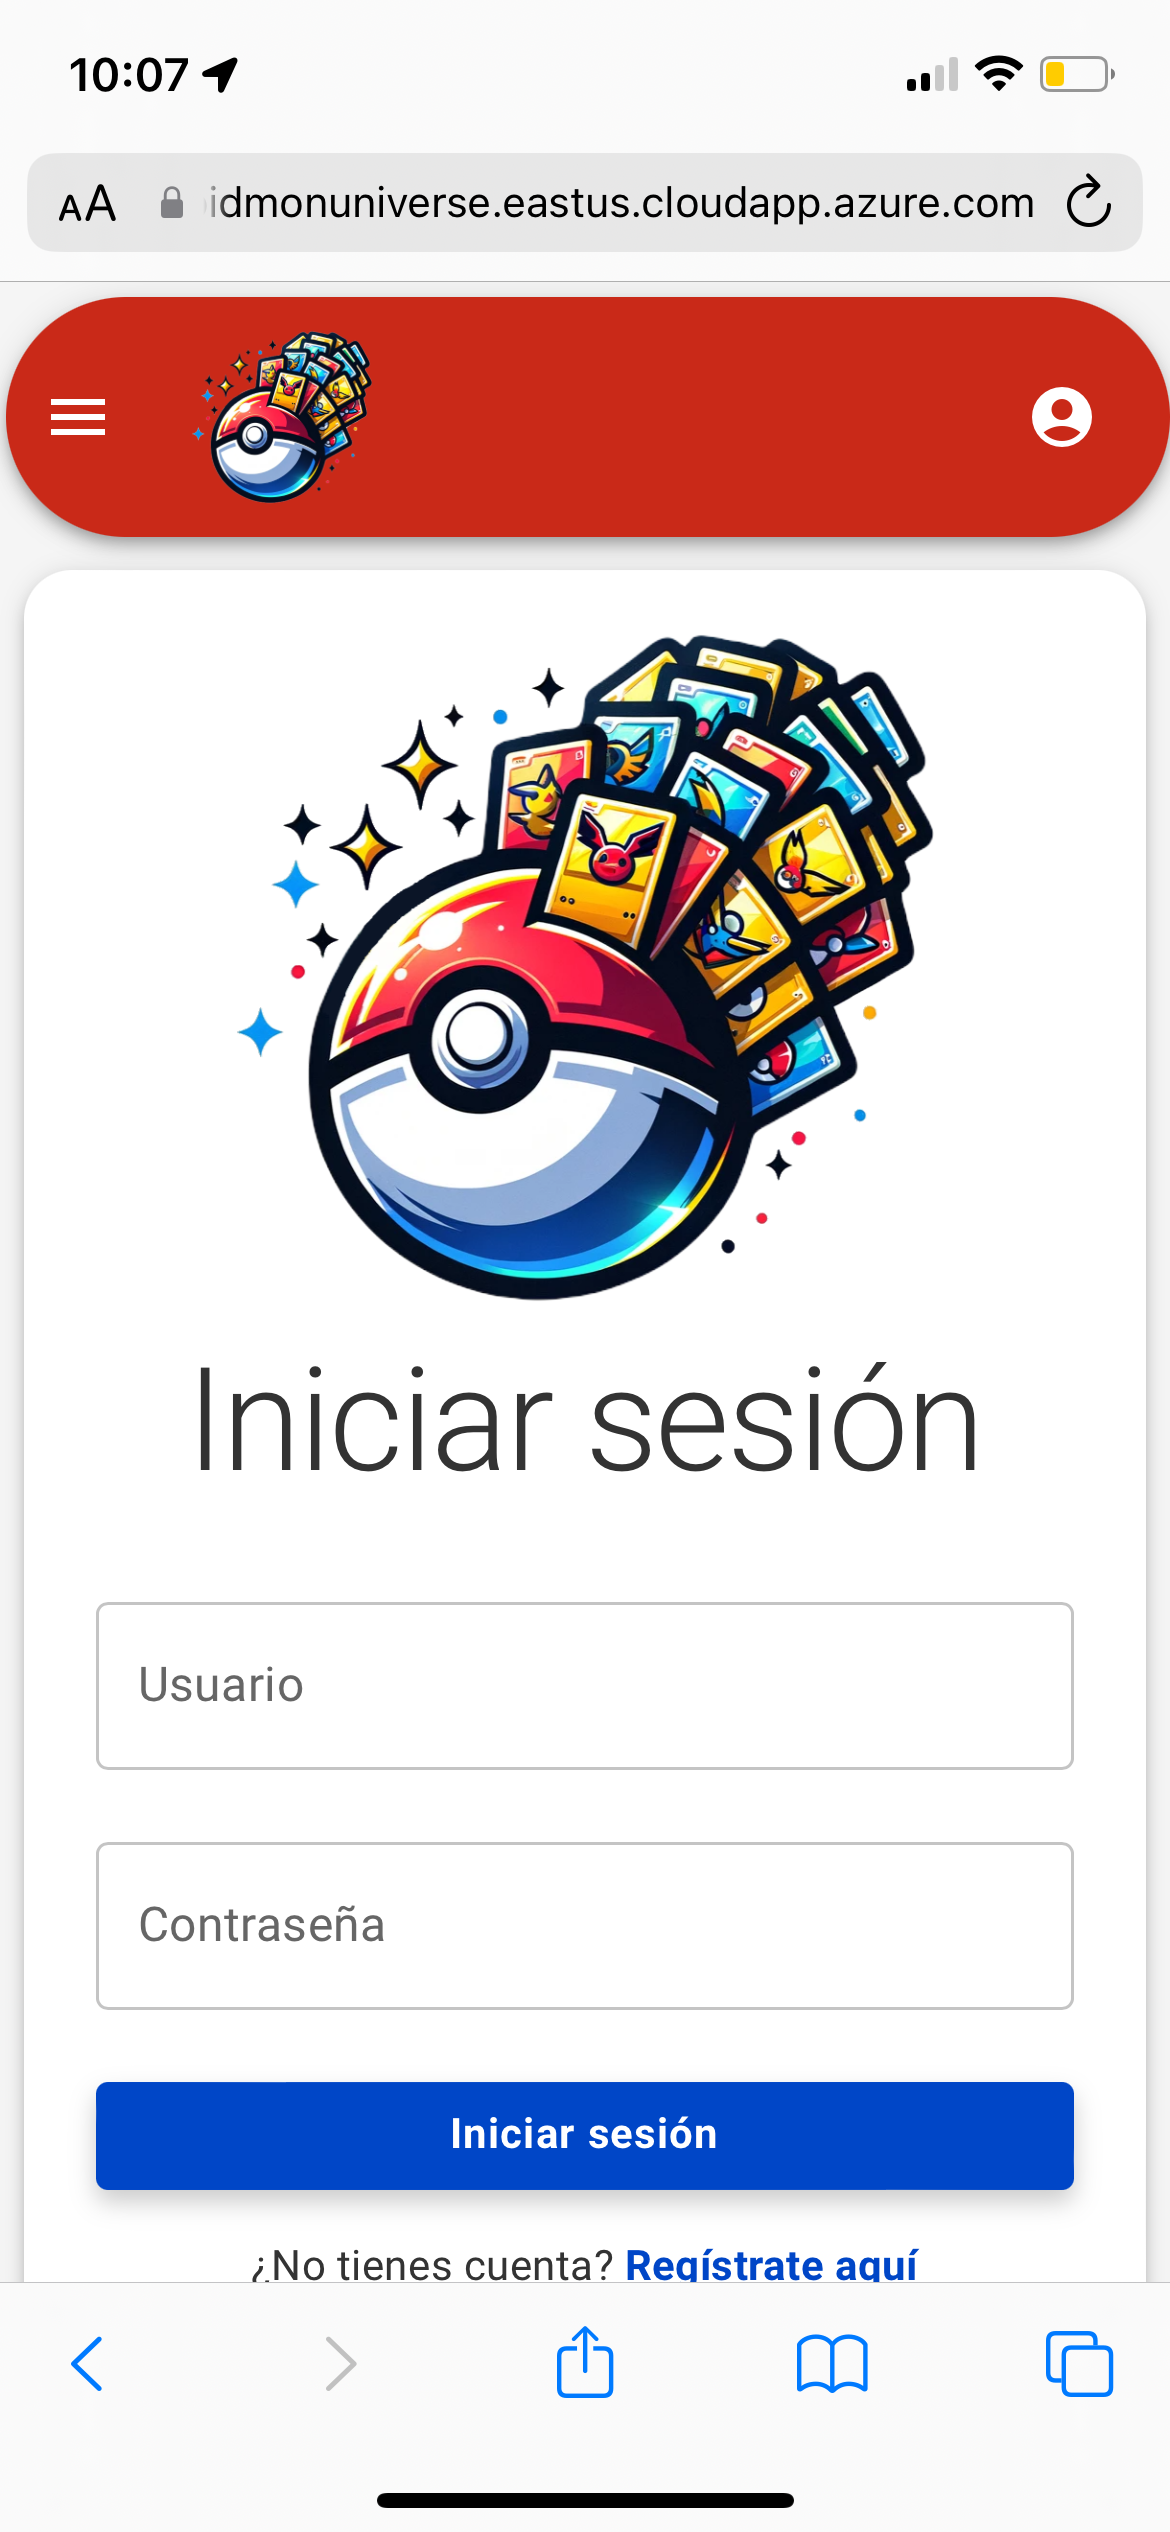
\includegraphics[ width=0.2\textwidth]{figures/adaptabilidad/login.png}
    \caption{Adaptabilidad Página Login}
    \label{fig:Adap-Login}
\end{figure}

\subsection*{Registro}
\begin{figure}[H]
    \centering
    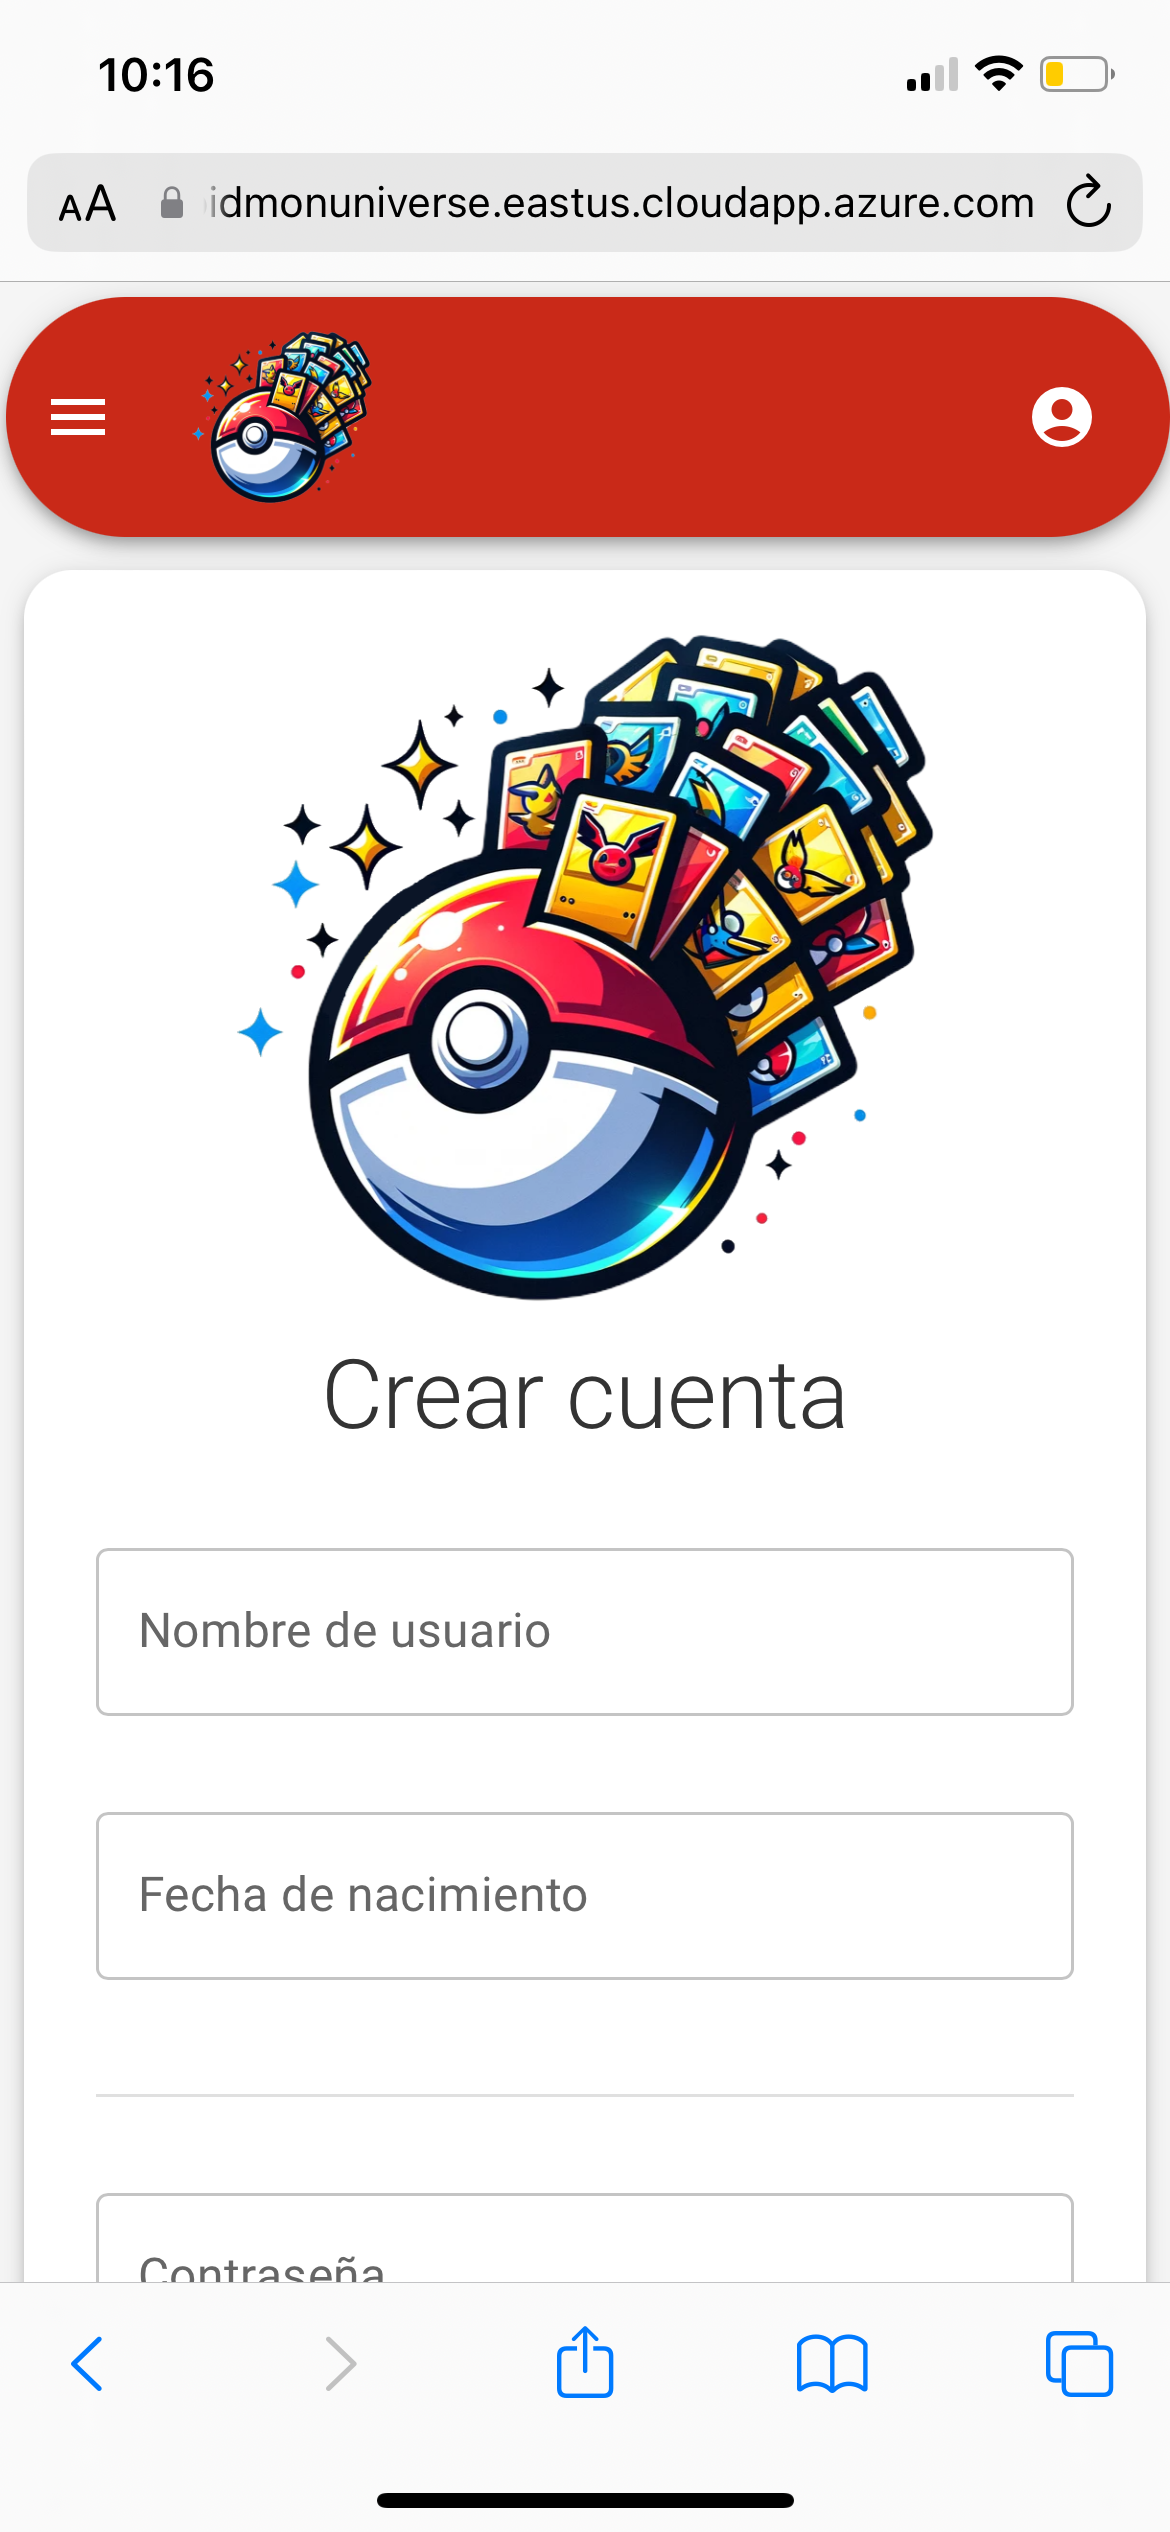
\includegraphics[ width=0.2\textwidth]{figures/adaptabilidad/registro.png}
    \caption{Adaptabilidad Página Registro}
    \label{fig:Adap-Registro}
\end{figure}

\subsection*{Acerca de}

\begin{figure}[H]
    \centering
    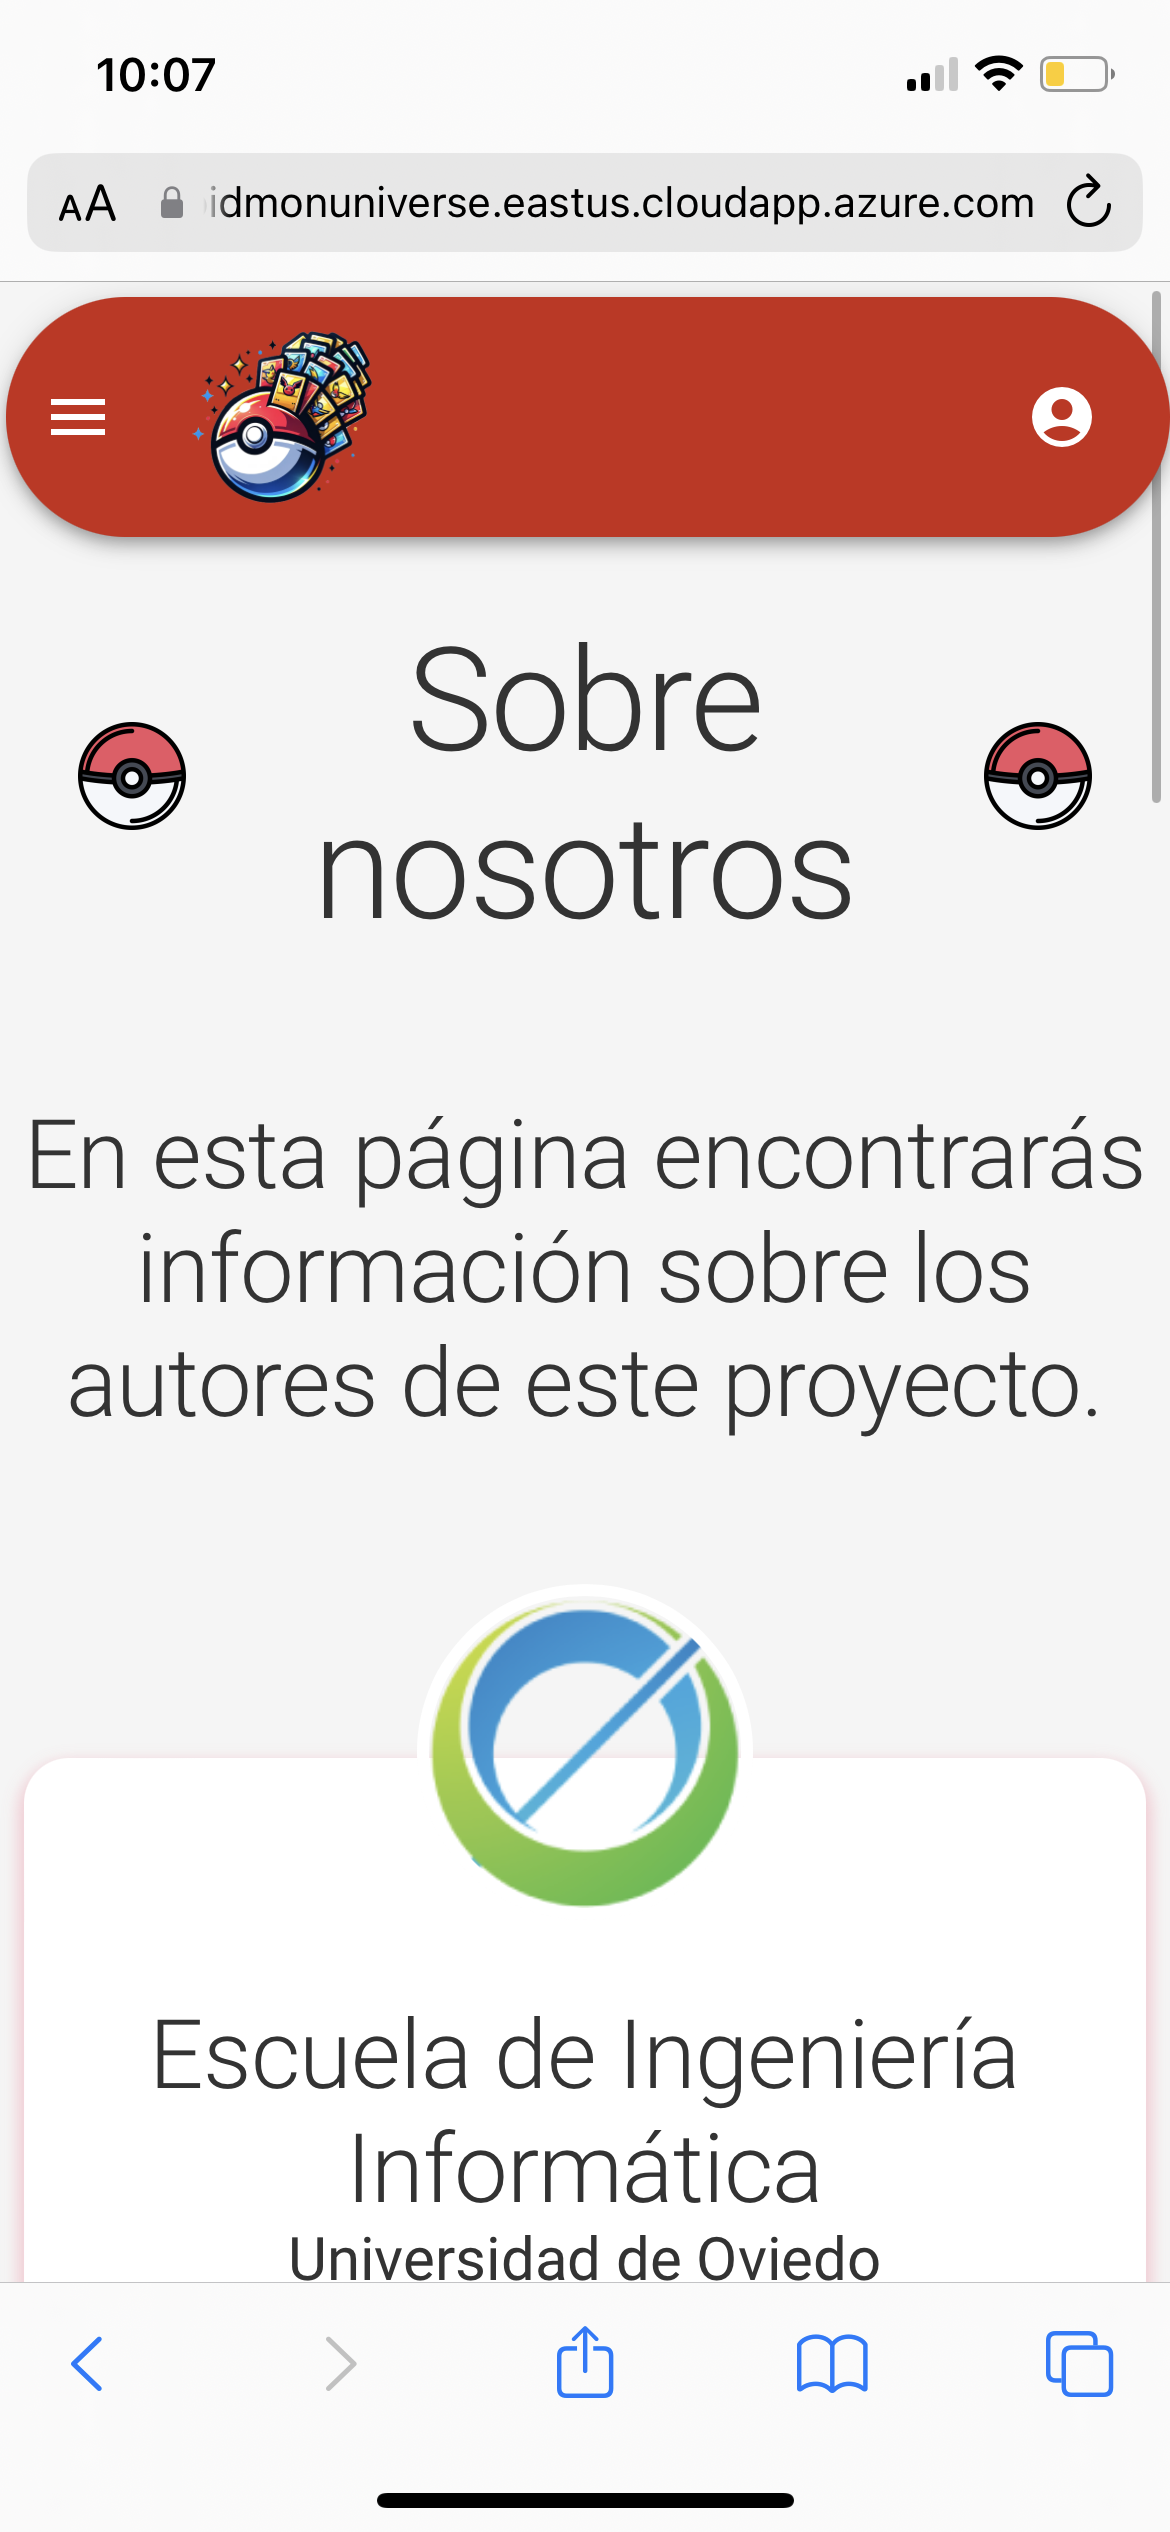
\includegraphics[width=0.2\textwidth]{figures/adaptabilidad/about.png}
    \caption{Adaptabilidad Página Acerca de}
    \label{fig:Adap-Acerca}
\end{figure}

\subsection*{Perfil}
\begin{figure}[H]
    \centering
    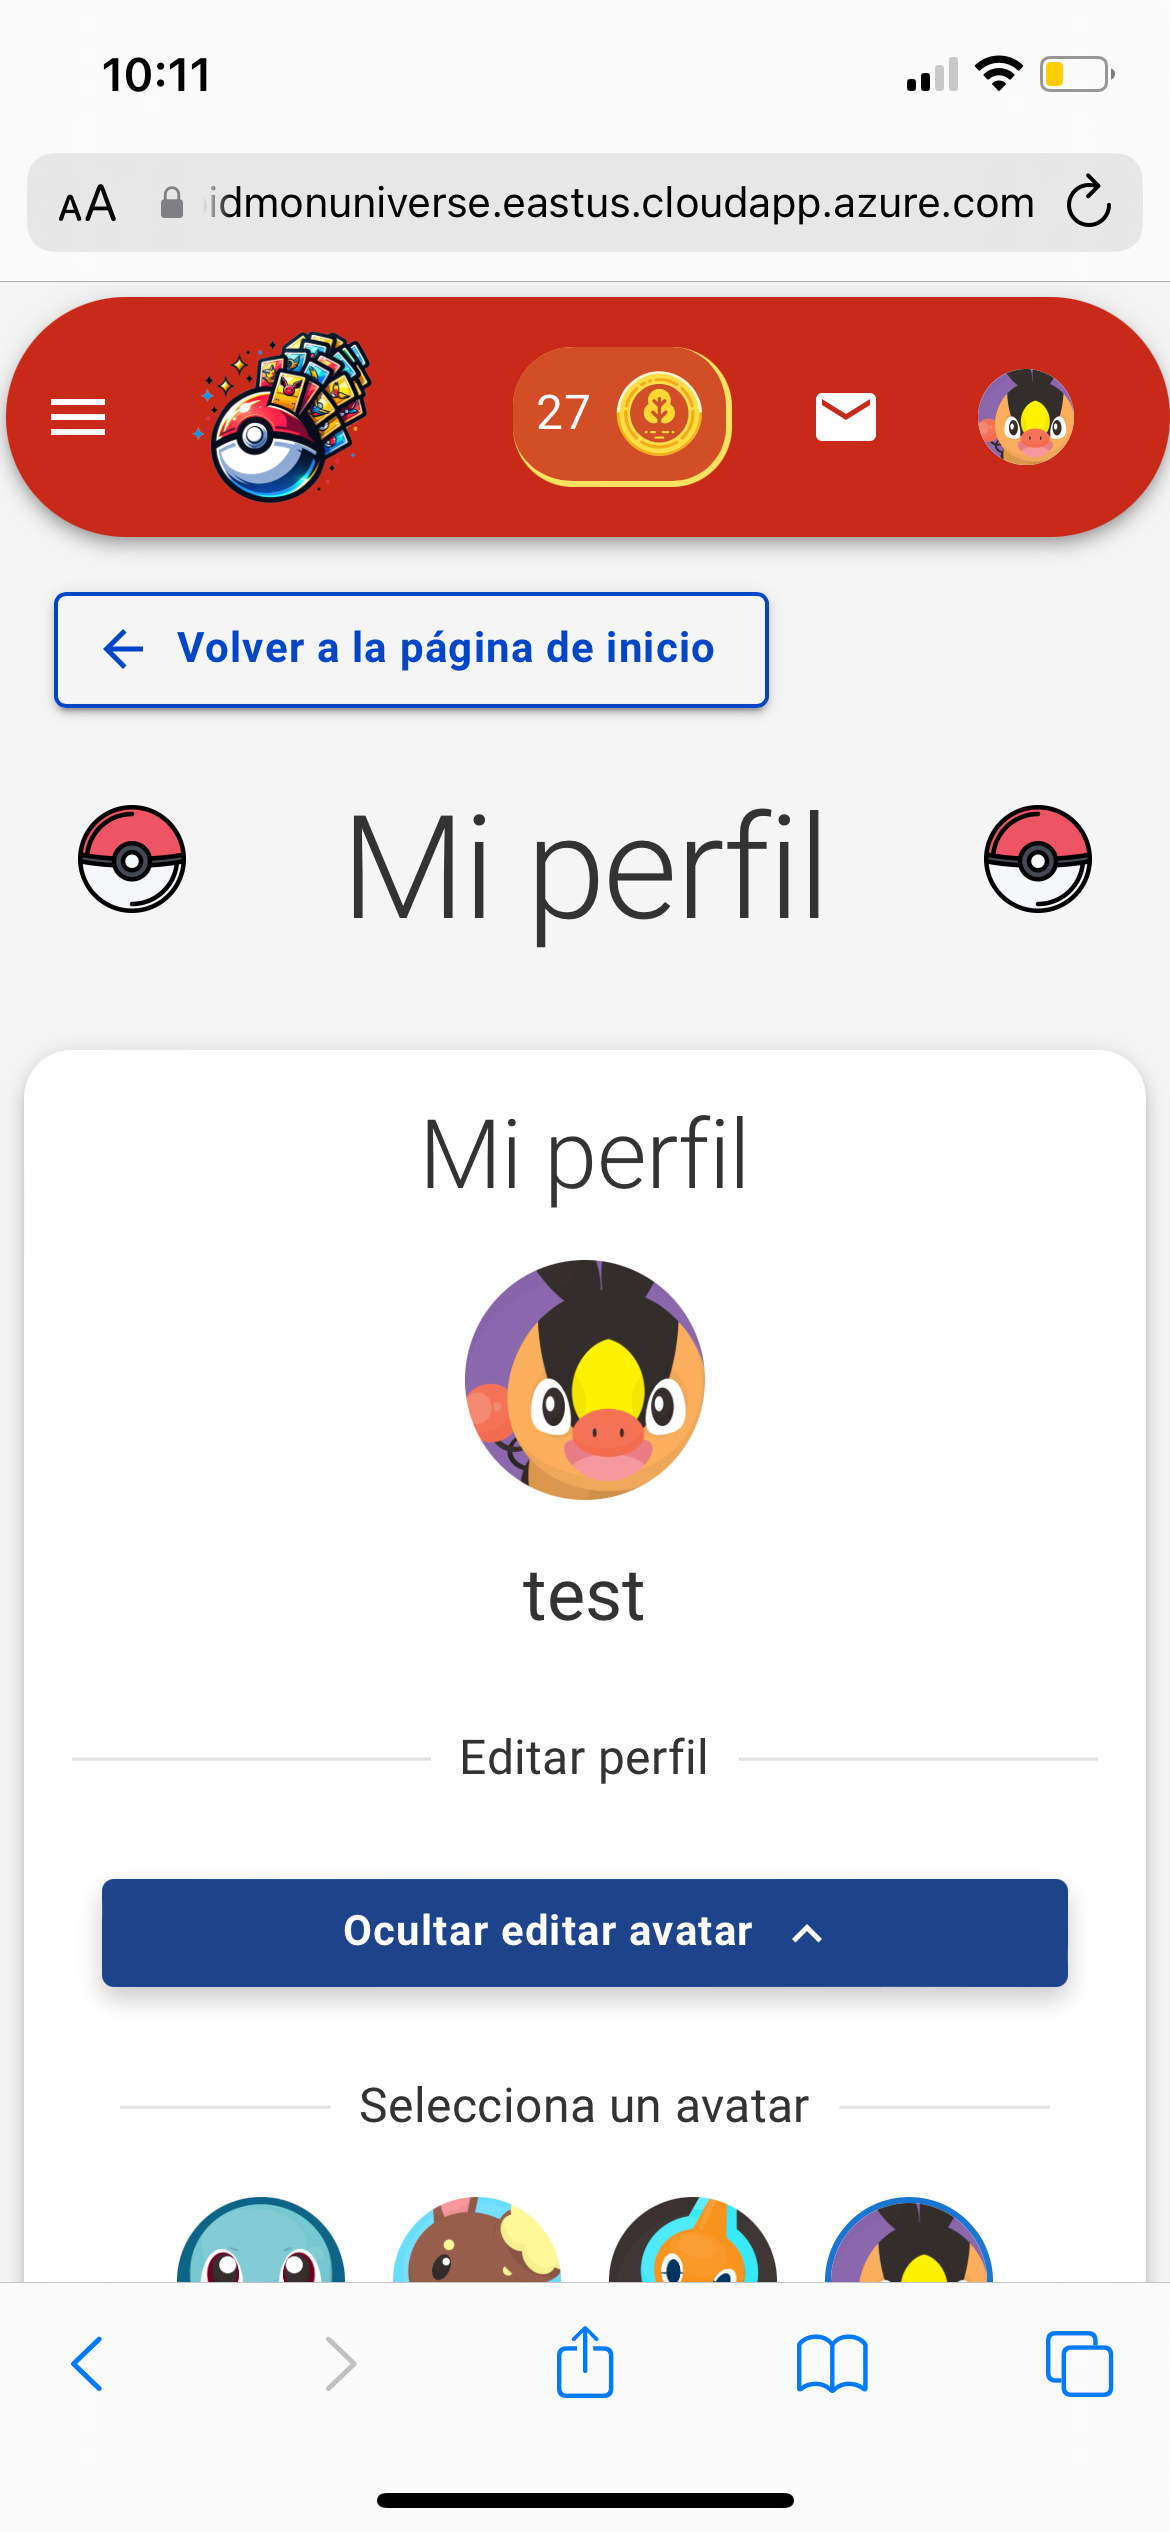
\includegraphics[ width=0.2\textwidth]{figures/adaptabilidad/perfil.png}
    \caption{Adaptabilidad Página Perfil}
    \label{fig:Adap-Perfil}
\end{figure}

\subsection*{Página principal de usuario autenticado}
\begin{figure}[H]
    \centering
    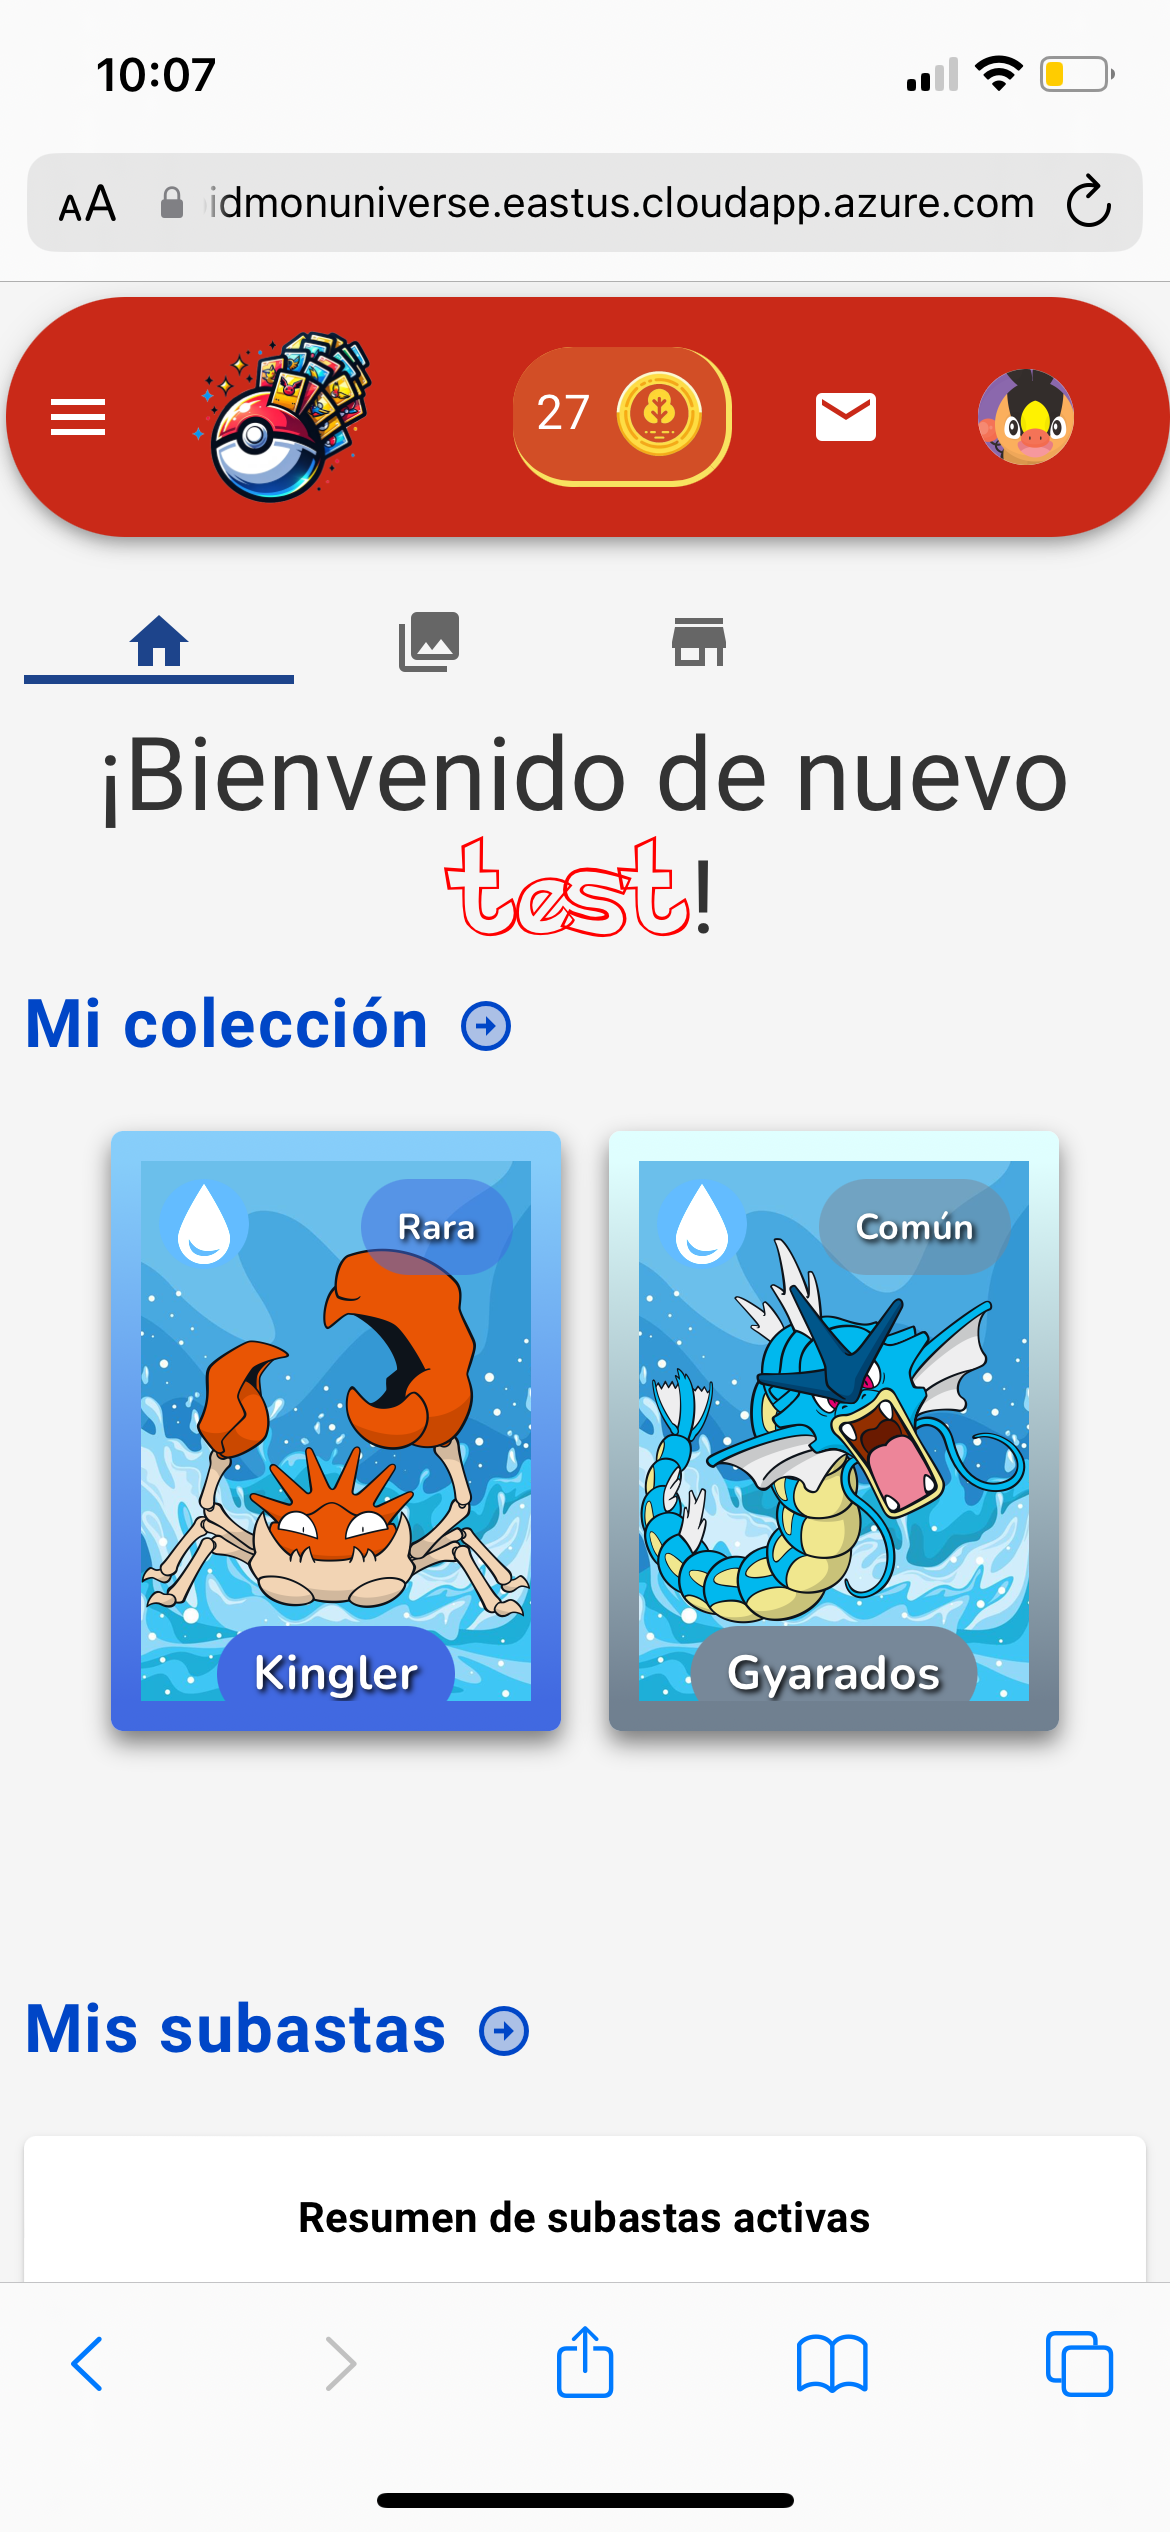
\includegraphics[width=0.2\textwidth]{figures/adaptabilidad/logued.png}
    \caption{Adaptabilidad Página principal de usuario autenticado}
    \label{fig:Adap-Principal-Usuario}
\end{figure}

\subsection*{Colección de cartas del usuario}
\begin{figure}[H]
    \centering
    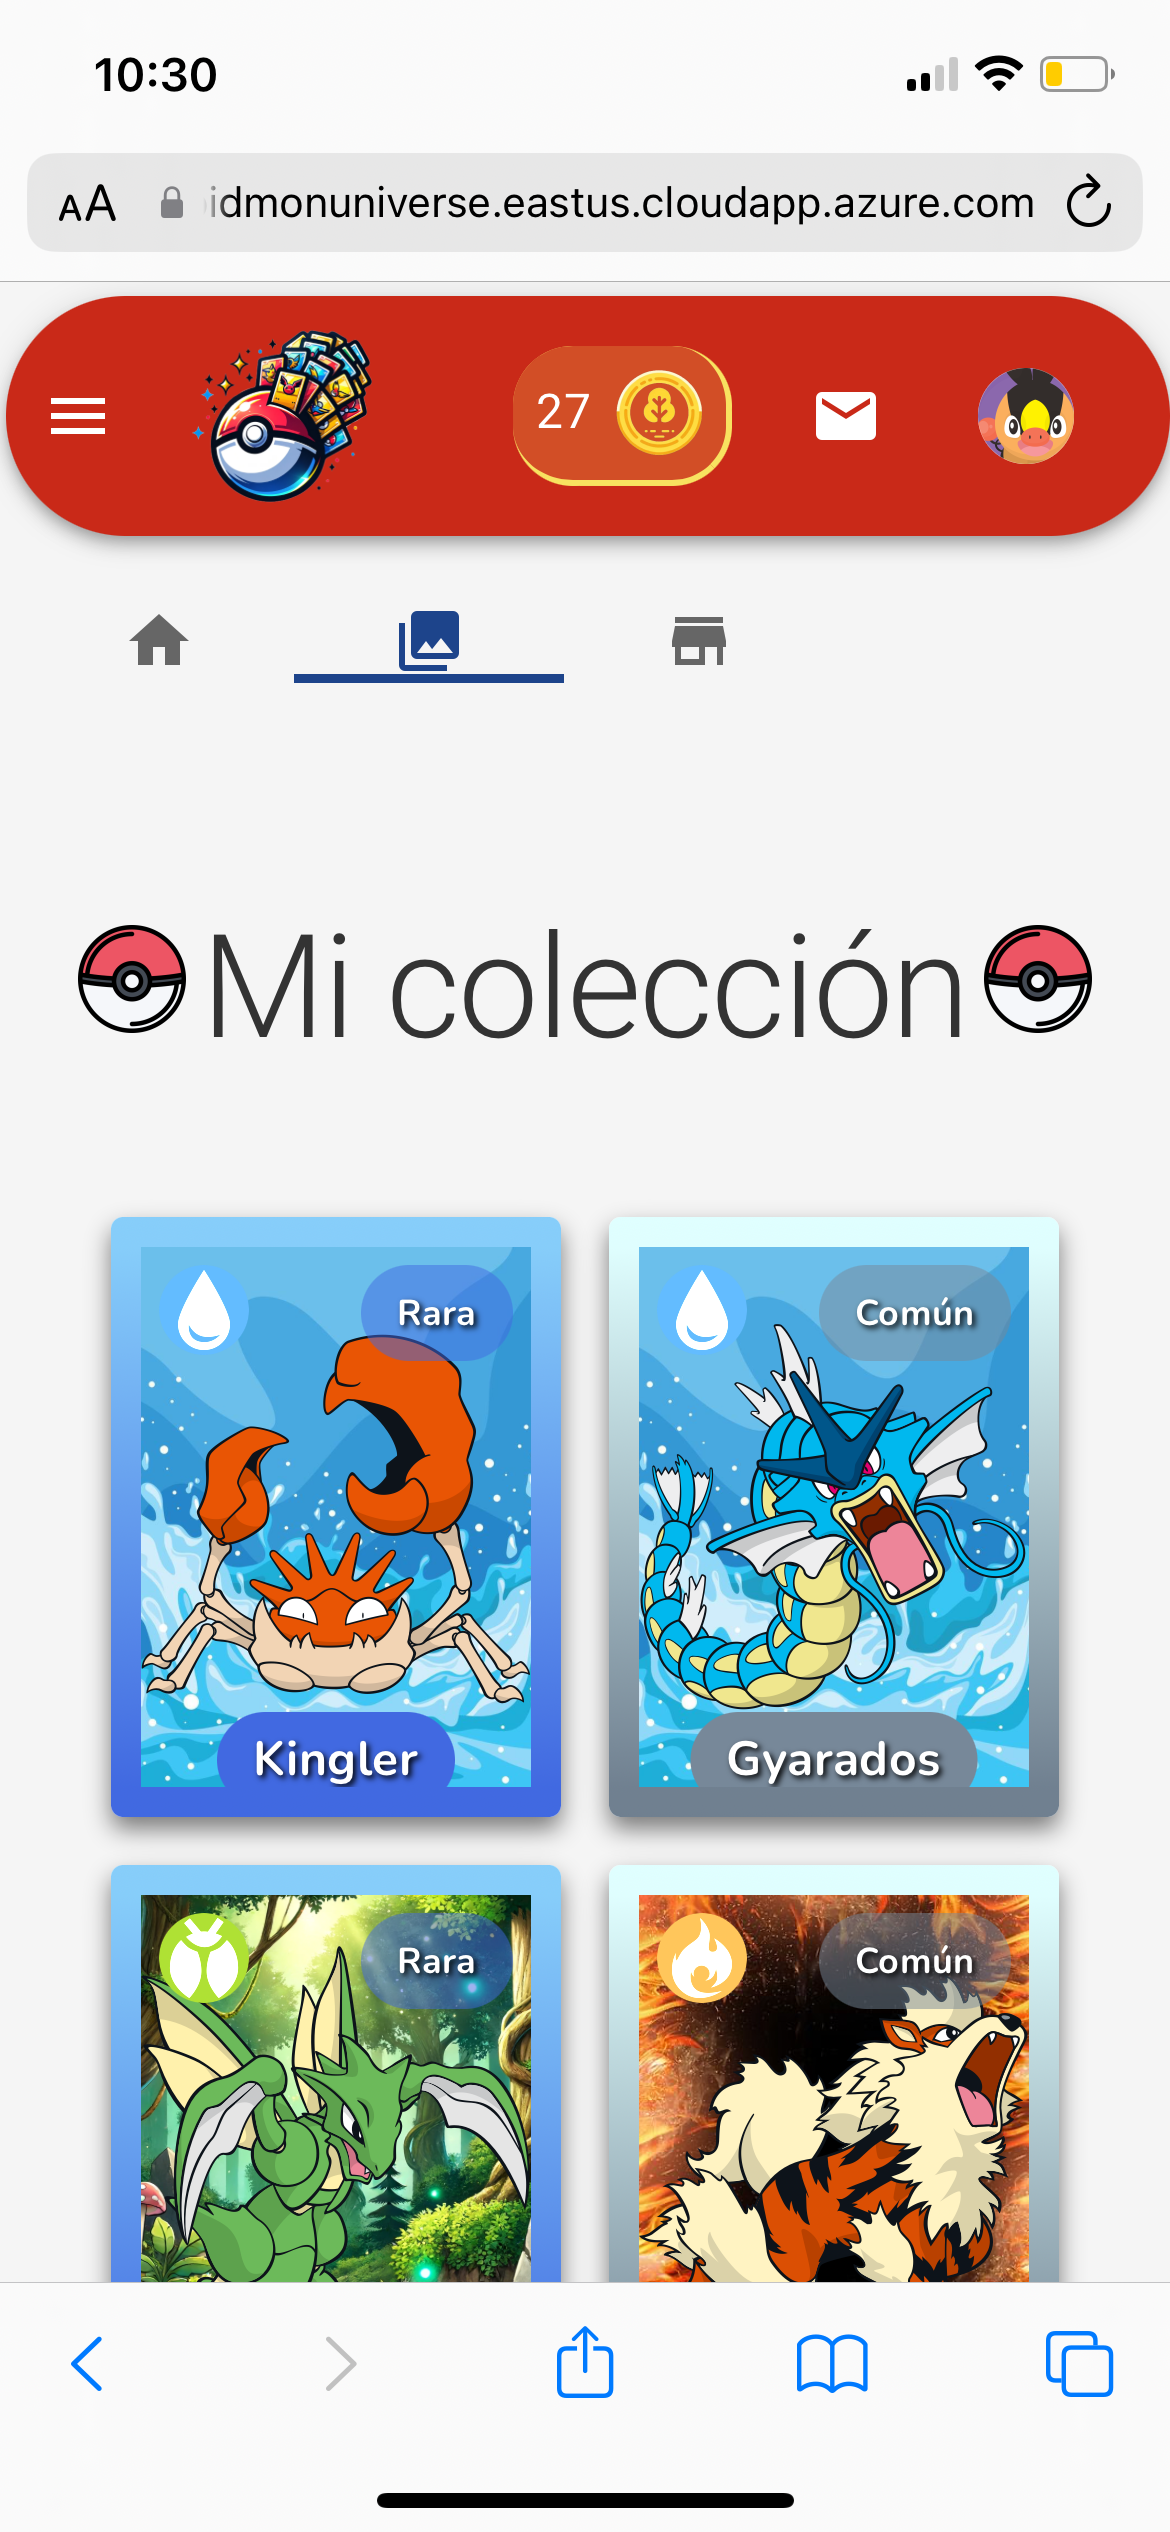
\includegraphics[width=0.2\textwidth]{figures/adaptabilidad/coleccion.png}
    \caption{Adaptabilidad Página Colección de cartas del usuario}
    \label{fig:Adap-Coleccion}
\end{figure}


\subsection*{Tienda}

\begin{figure}[H]
    \centering
    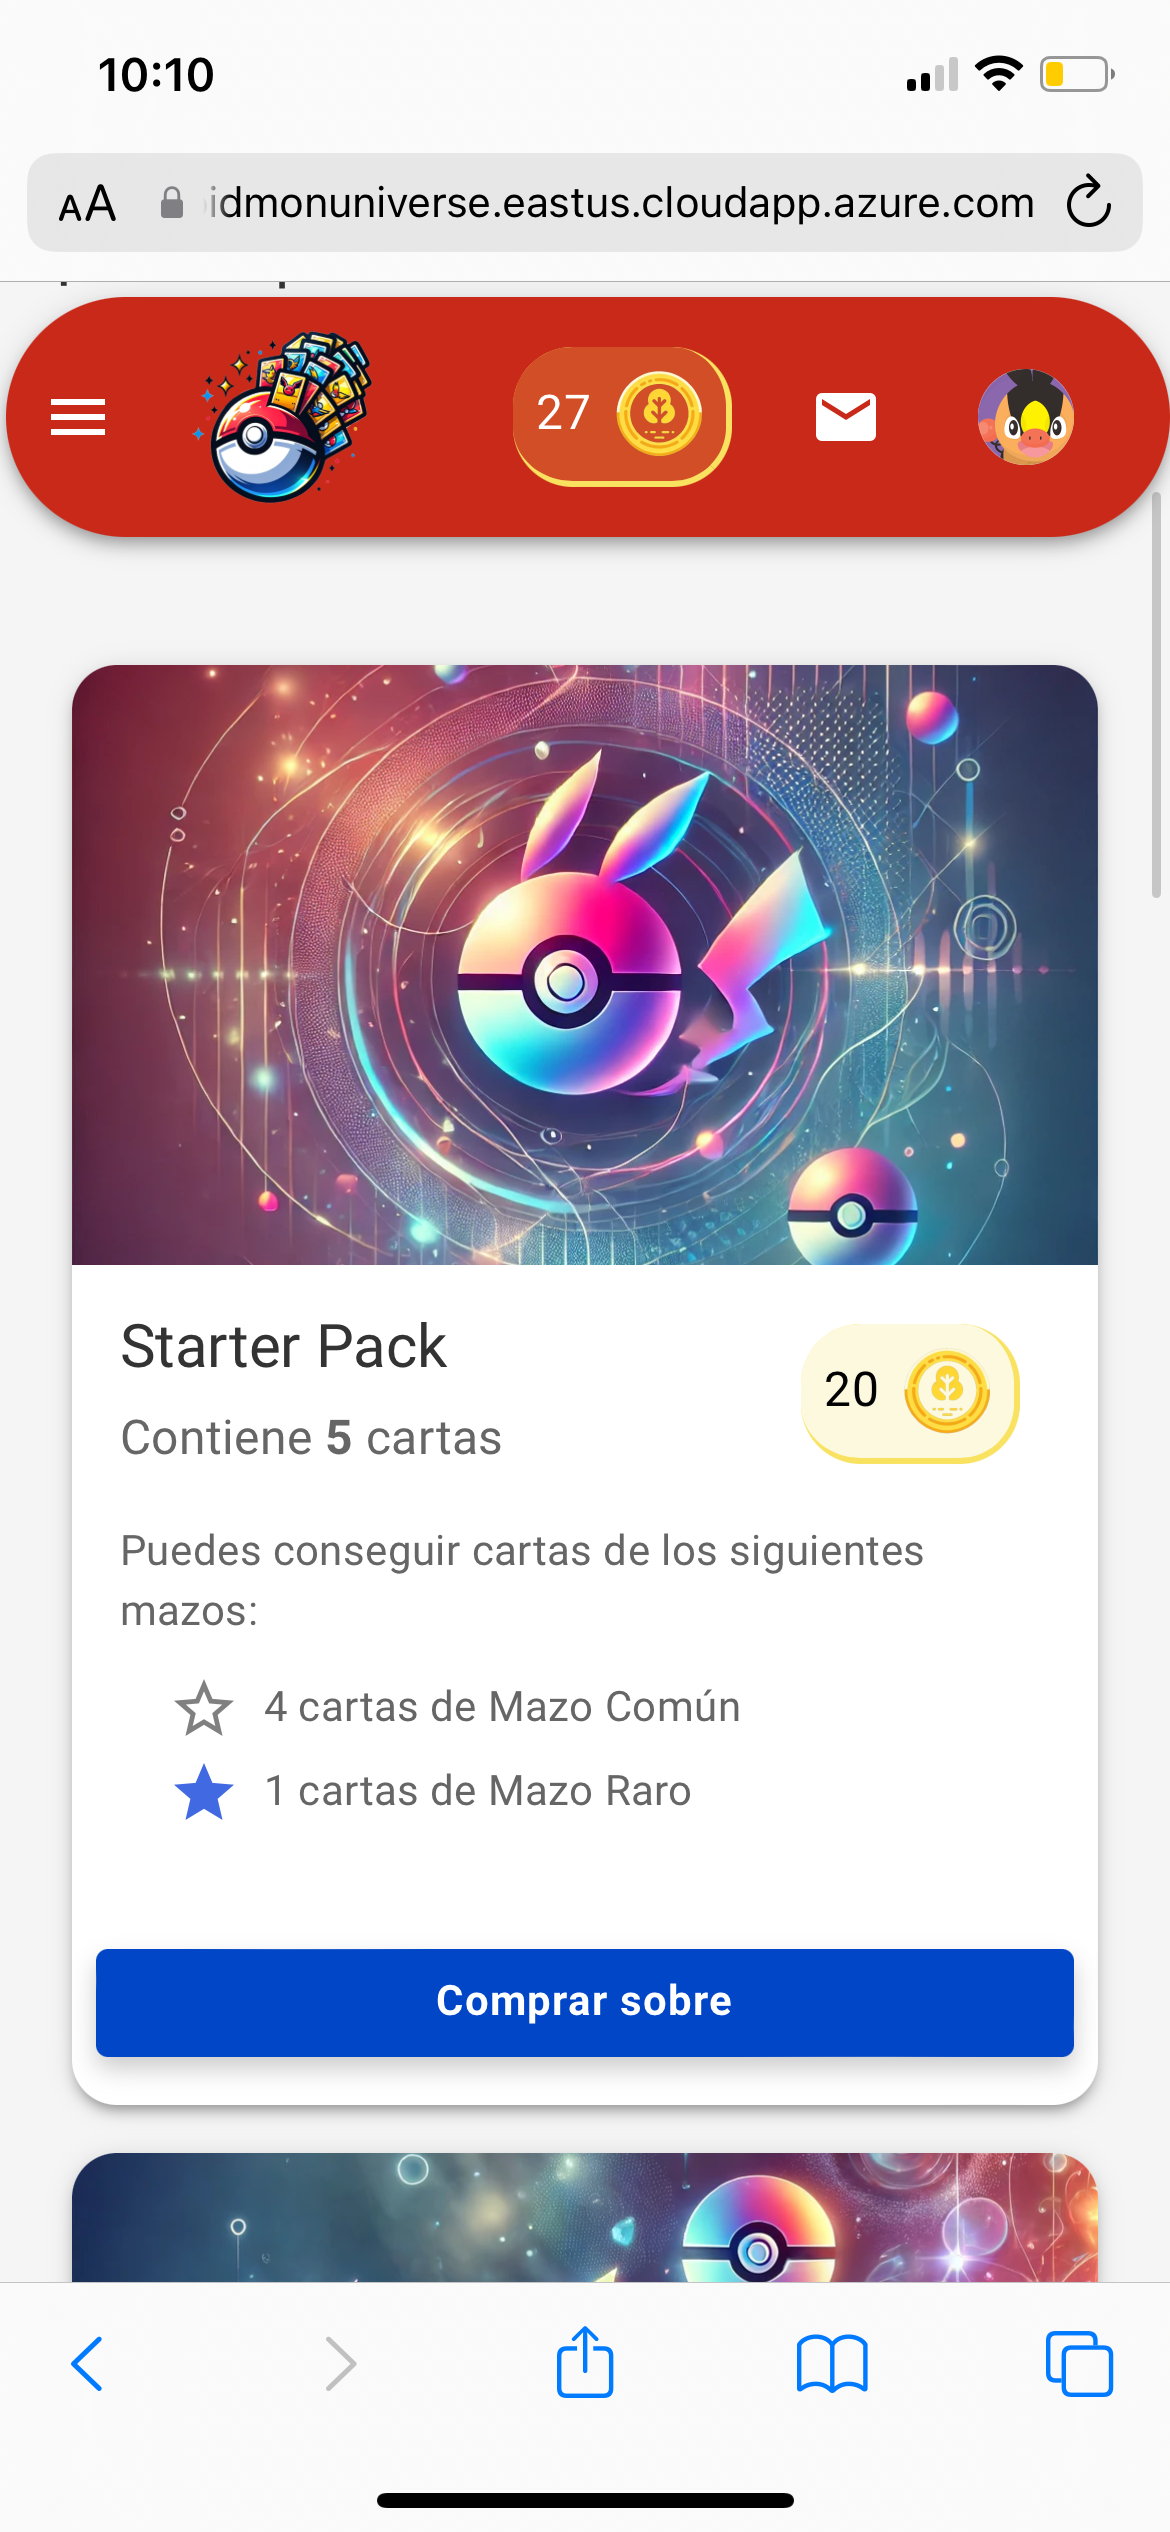
\includegraphics[ width=0.2\textwidth]{figures/adaptabilidad/tienda.png}
    \caption{Adaptabilidad Página Tienda}
    \label{fig:Adap-Tienda}
\end{figure}


\subsection*{Detalle de una carta}
\begin{figure}[H]
    \centering
    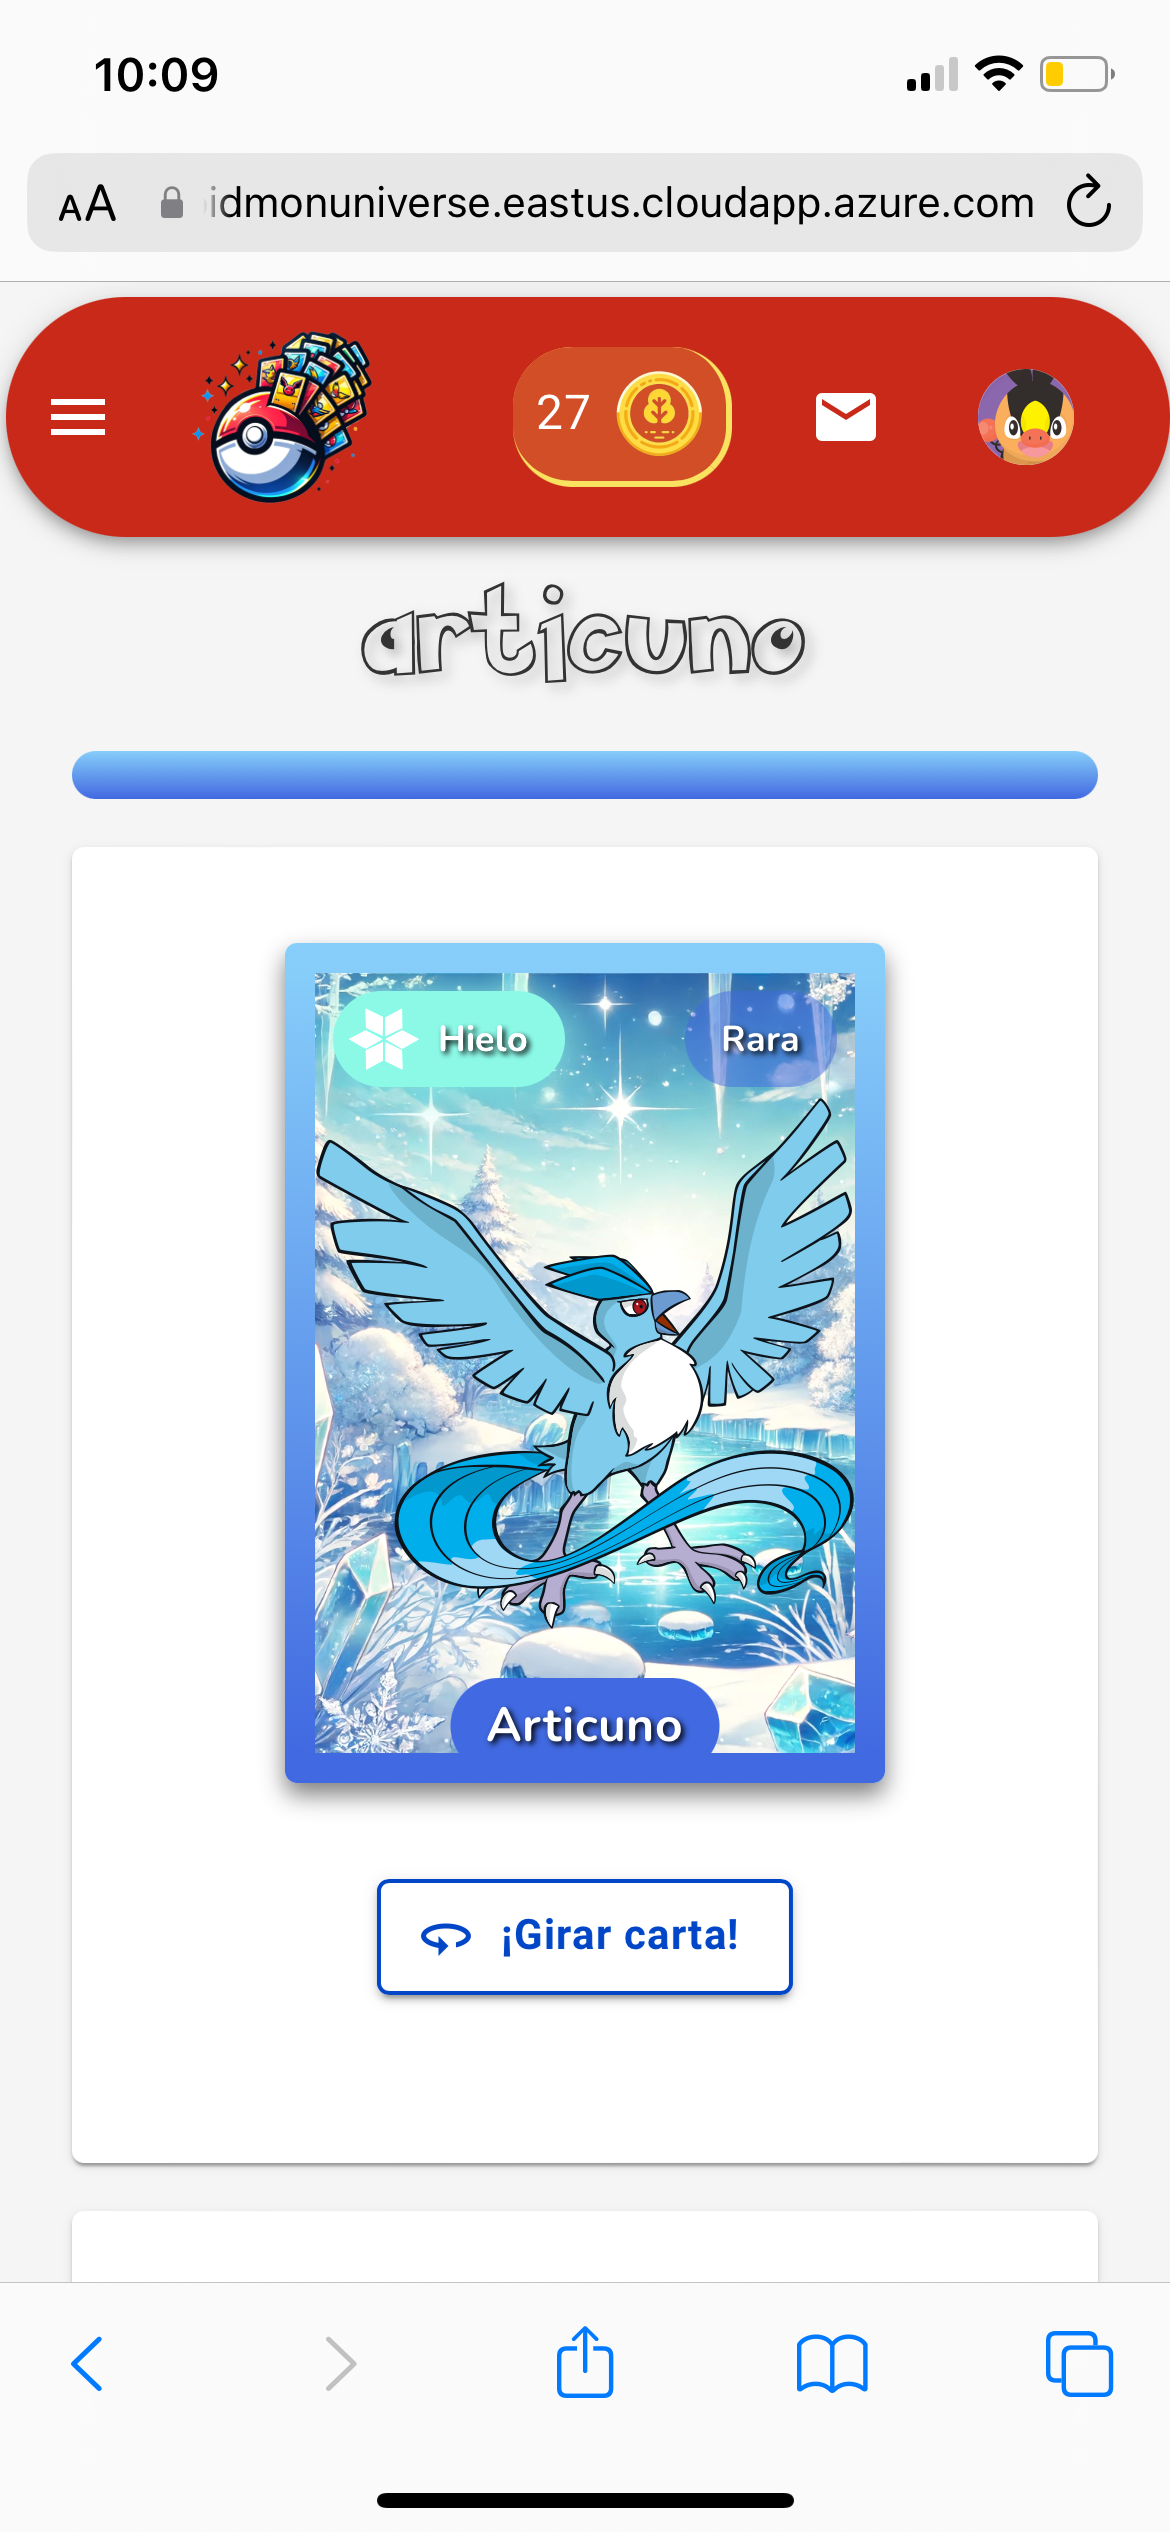
\includegraphics[width=0.2\textwidth]{figures/adaptabilidad/detalle_carta.png}
    \caption{Adaptabilidad Página Detalle de una carta}
    \label{fig:Adap-Carta}  
\end{figure}

\subsection*{Subastas activas}
\begin{figure}[H]
    \centering
    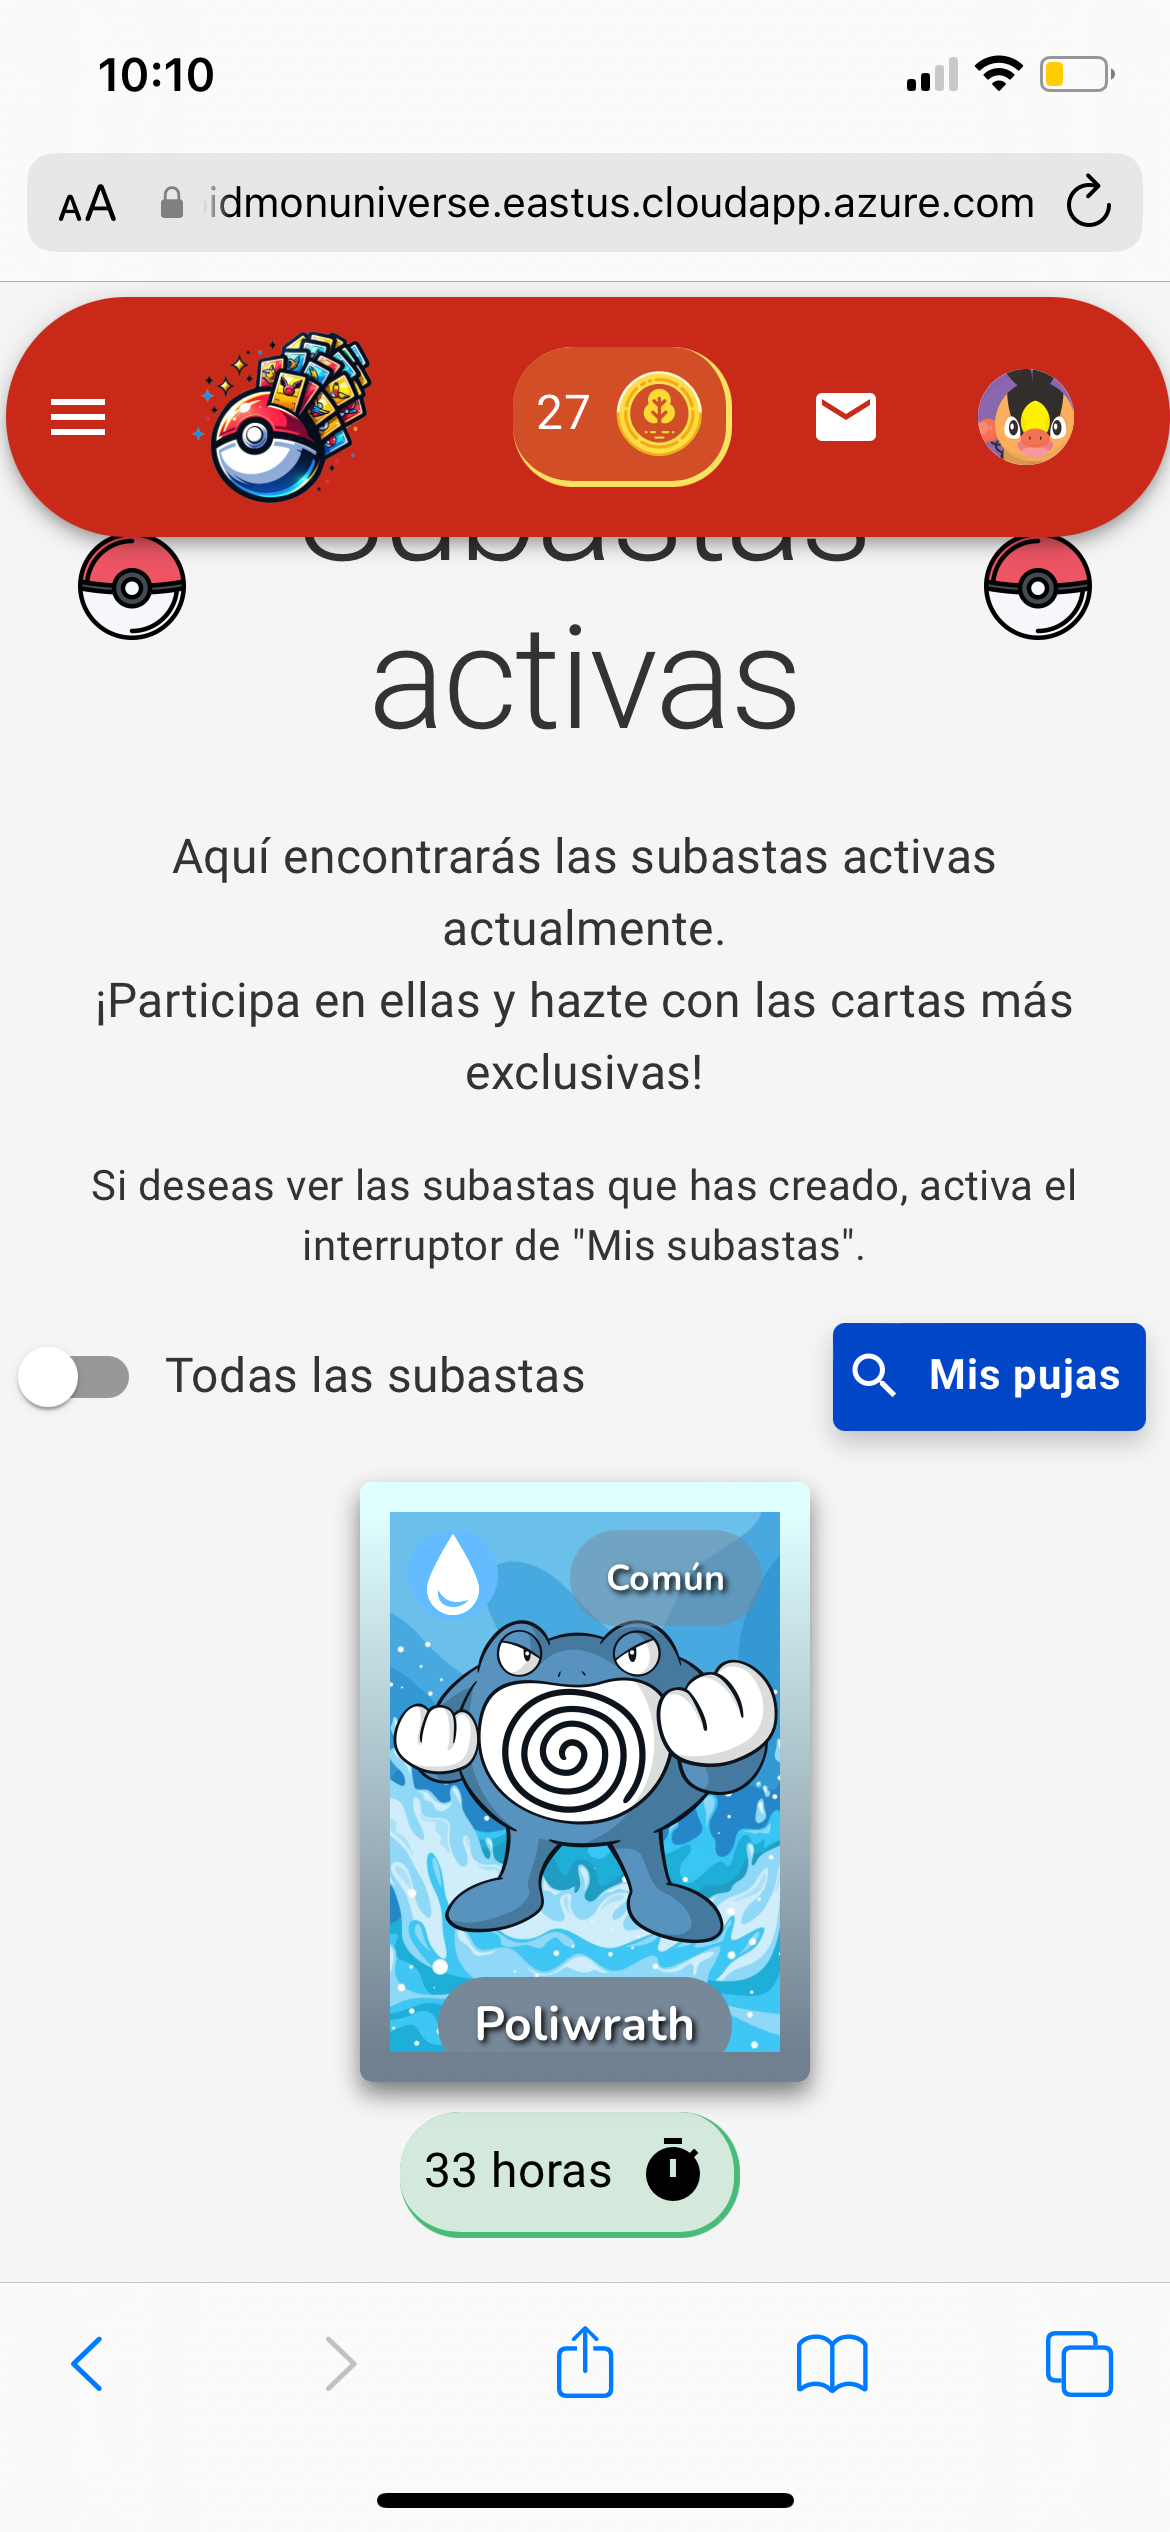
\includegraphics[width=0.2\textwidth]{figures/adaptabilidad/subastas.png}
    \caption{Adaptabilidad Página Subastas activas}
    \label{fig:Adap-Subastas}
\end{figure}


\subsection*{Detalle de una subasta}
\begin{figure}[H]
    \centering
    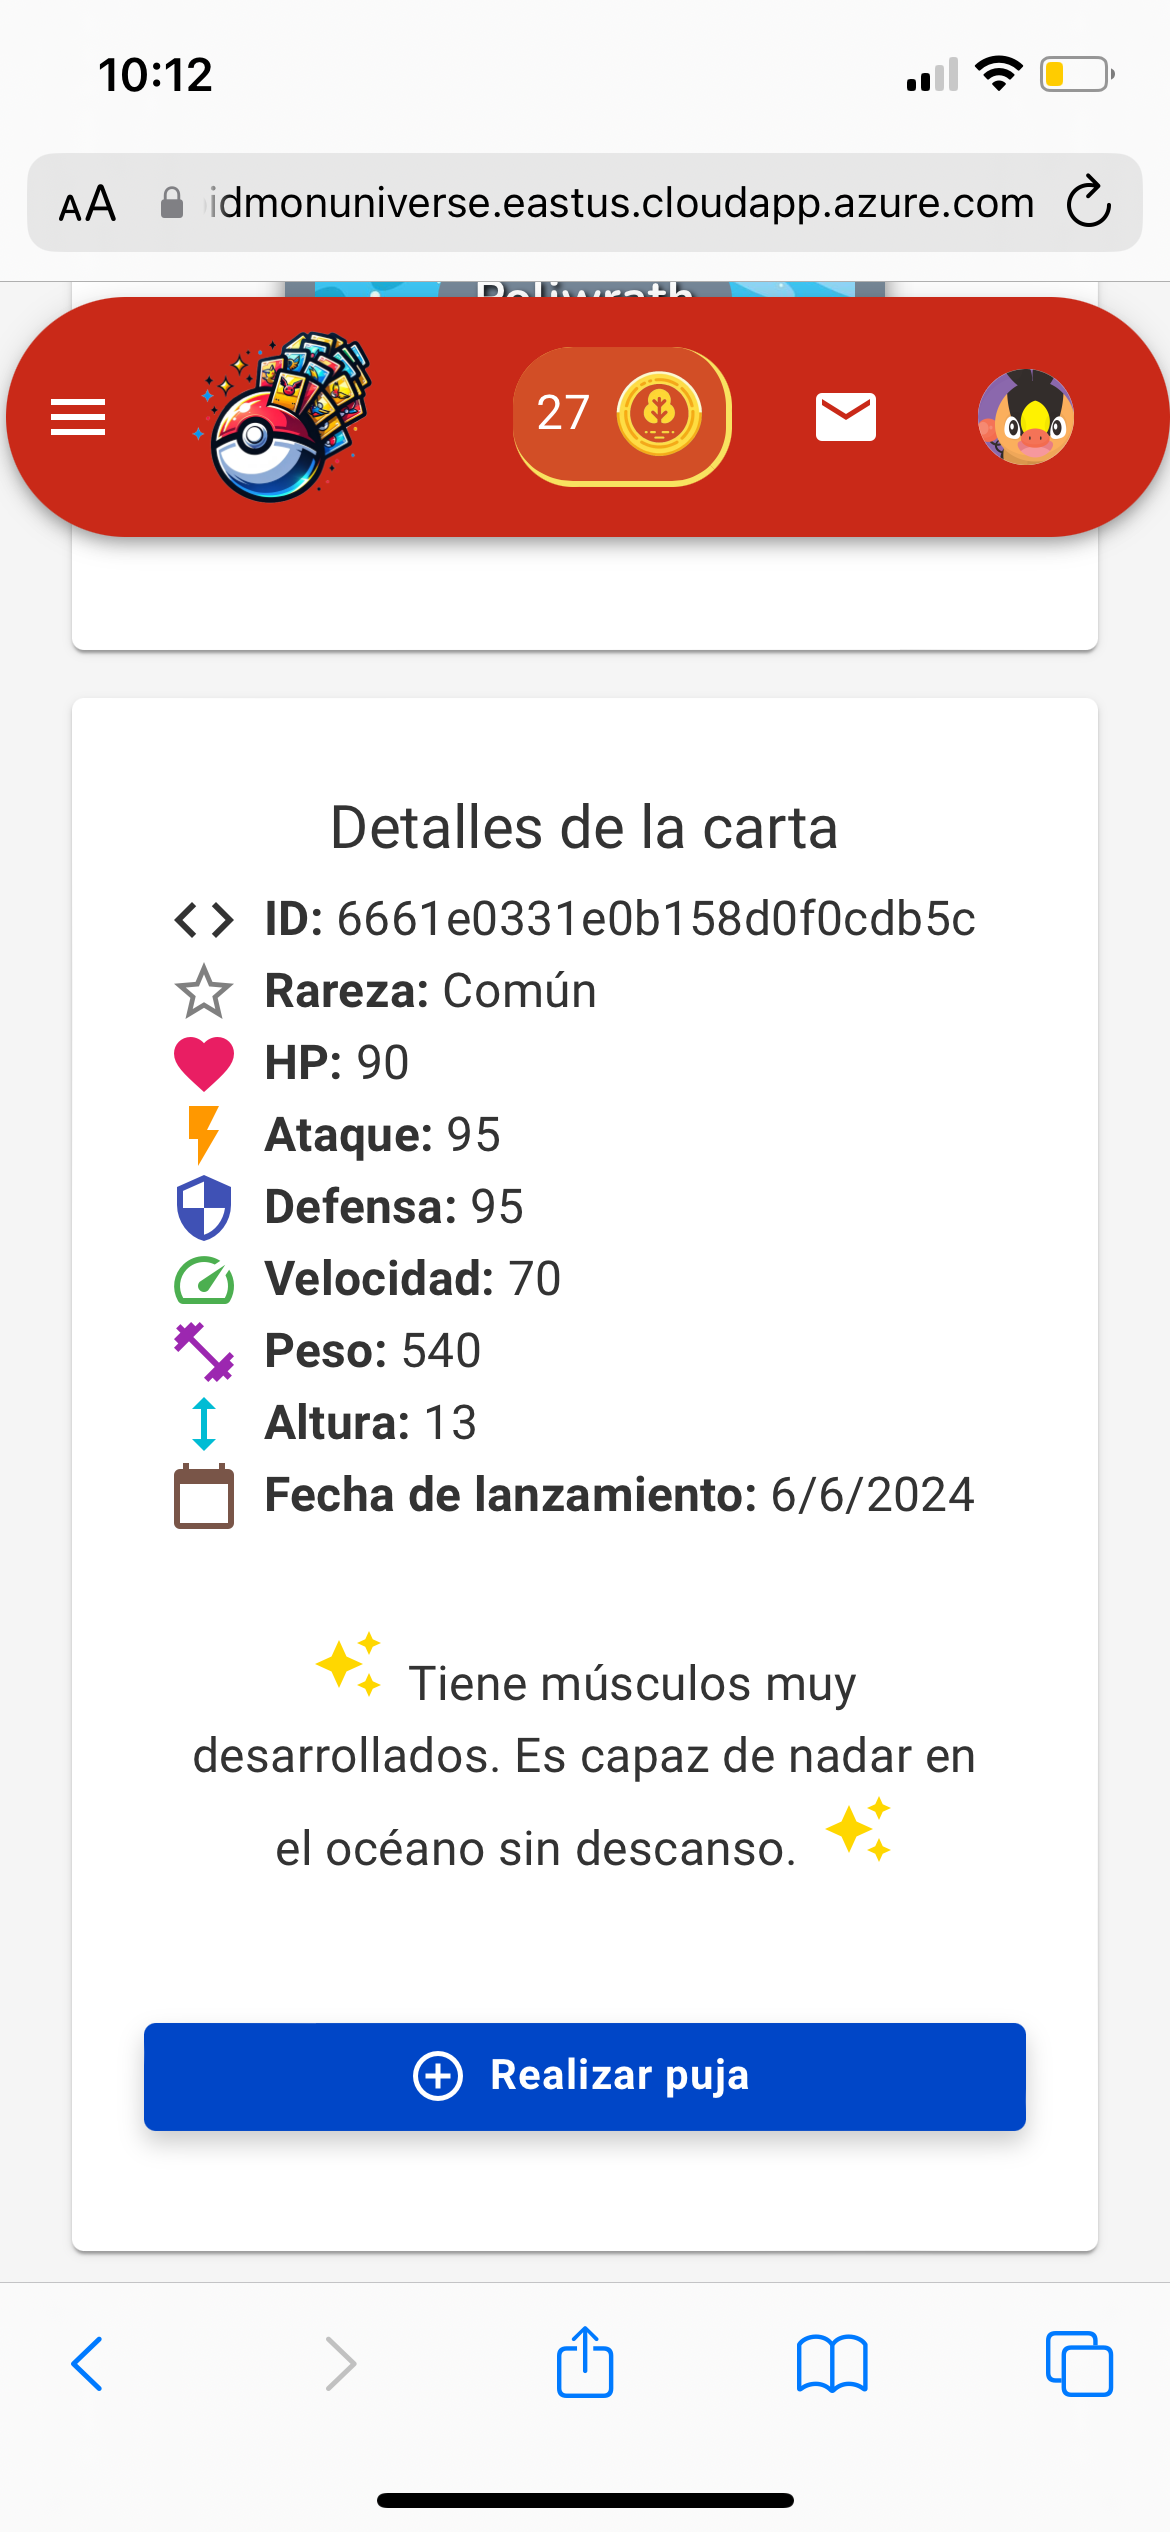
\includegraphics[width=0.2\textwidth]{figures/adaptabilidad/detalle_subasta.png}
    \caption{Adaptabilidad Página Detalle de una subasta}
    \label{fig:Adap-Detalle-Subasta}
\end{figure}

\subsection*{Subastas propias}
\begin{figure}[H]
    \centering
    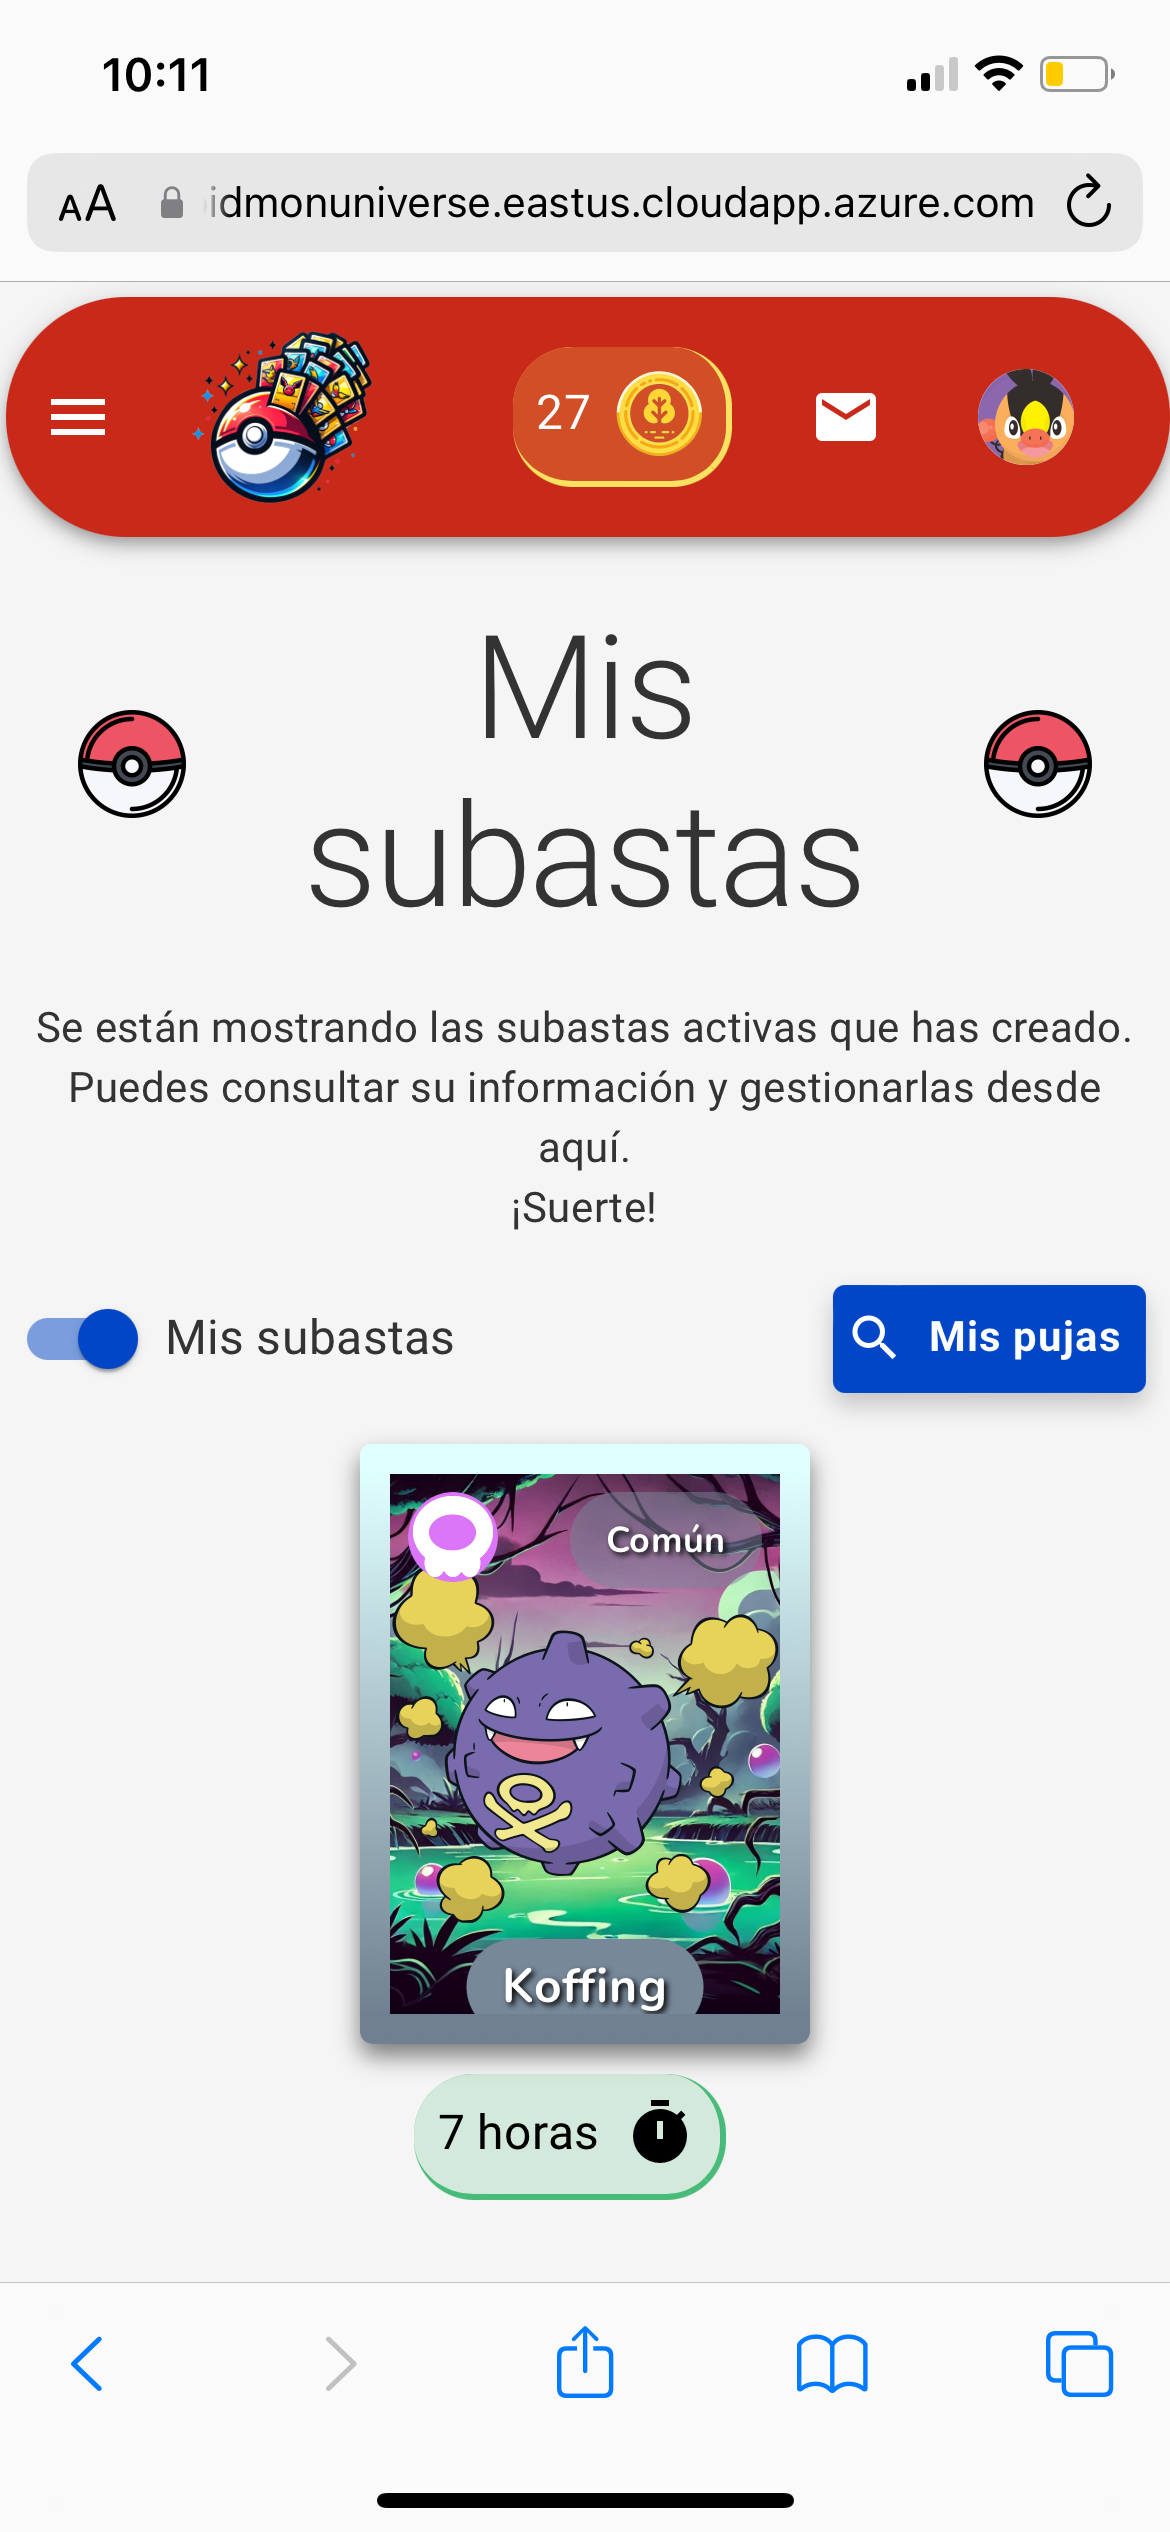
\includegraphics[width=0.2\textwidth]{figures/adaptabilidad/mis_subastas.png}
    \caption{Adaptabilidad Página Subastas propias}
    \label{fig:Adap-Mis-Subastas}
\end{figure}

\subsection*{Mis pujas activas}
\begin{figure}[H]
    \centering
    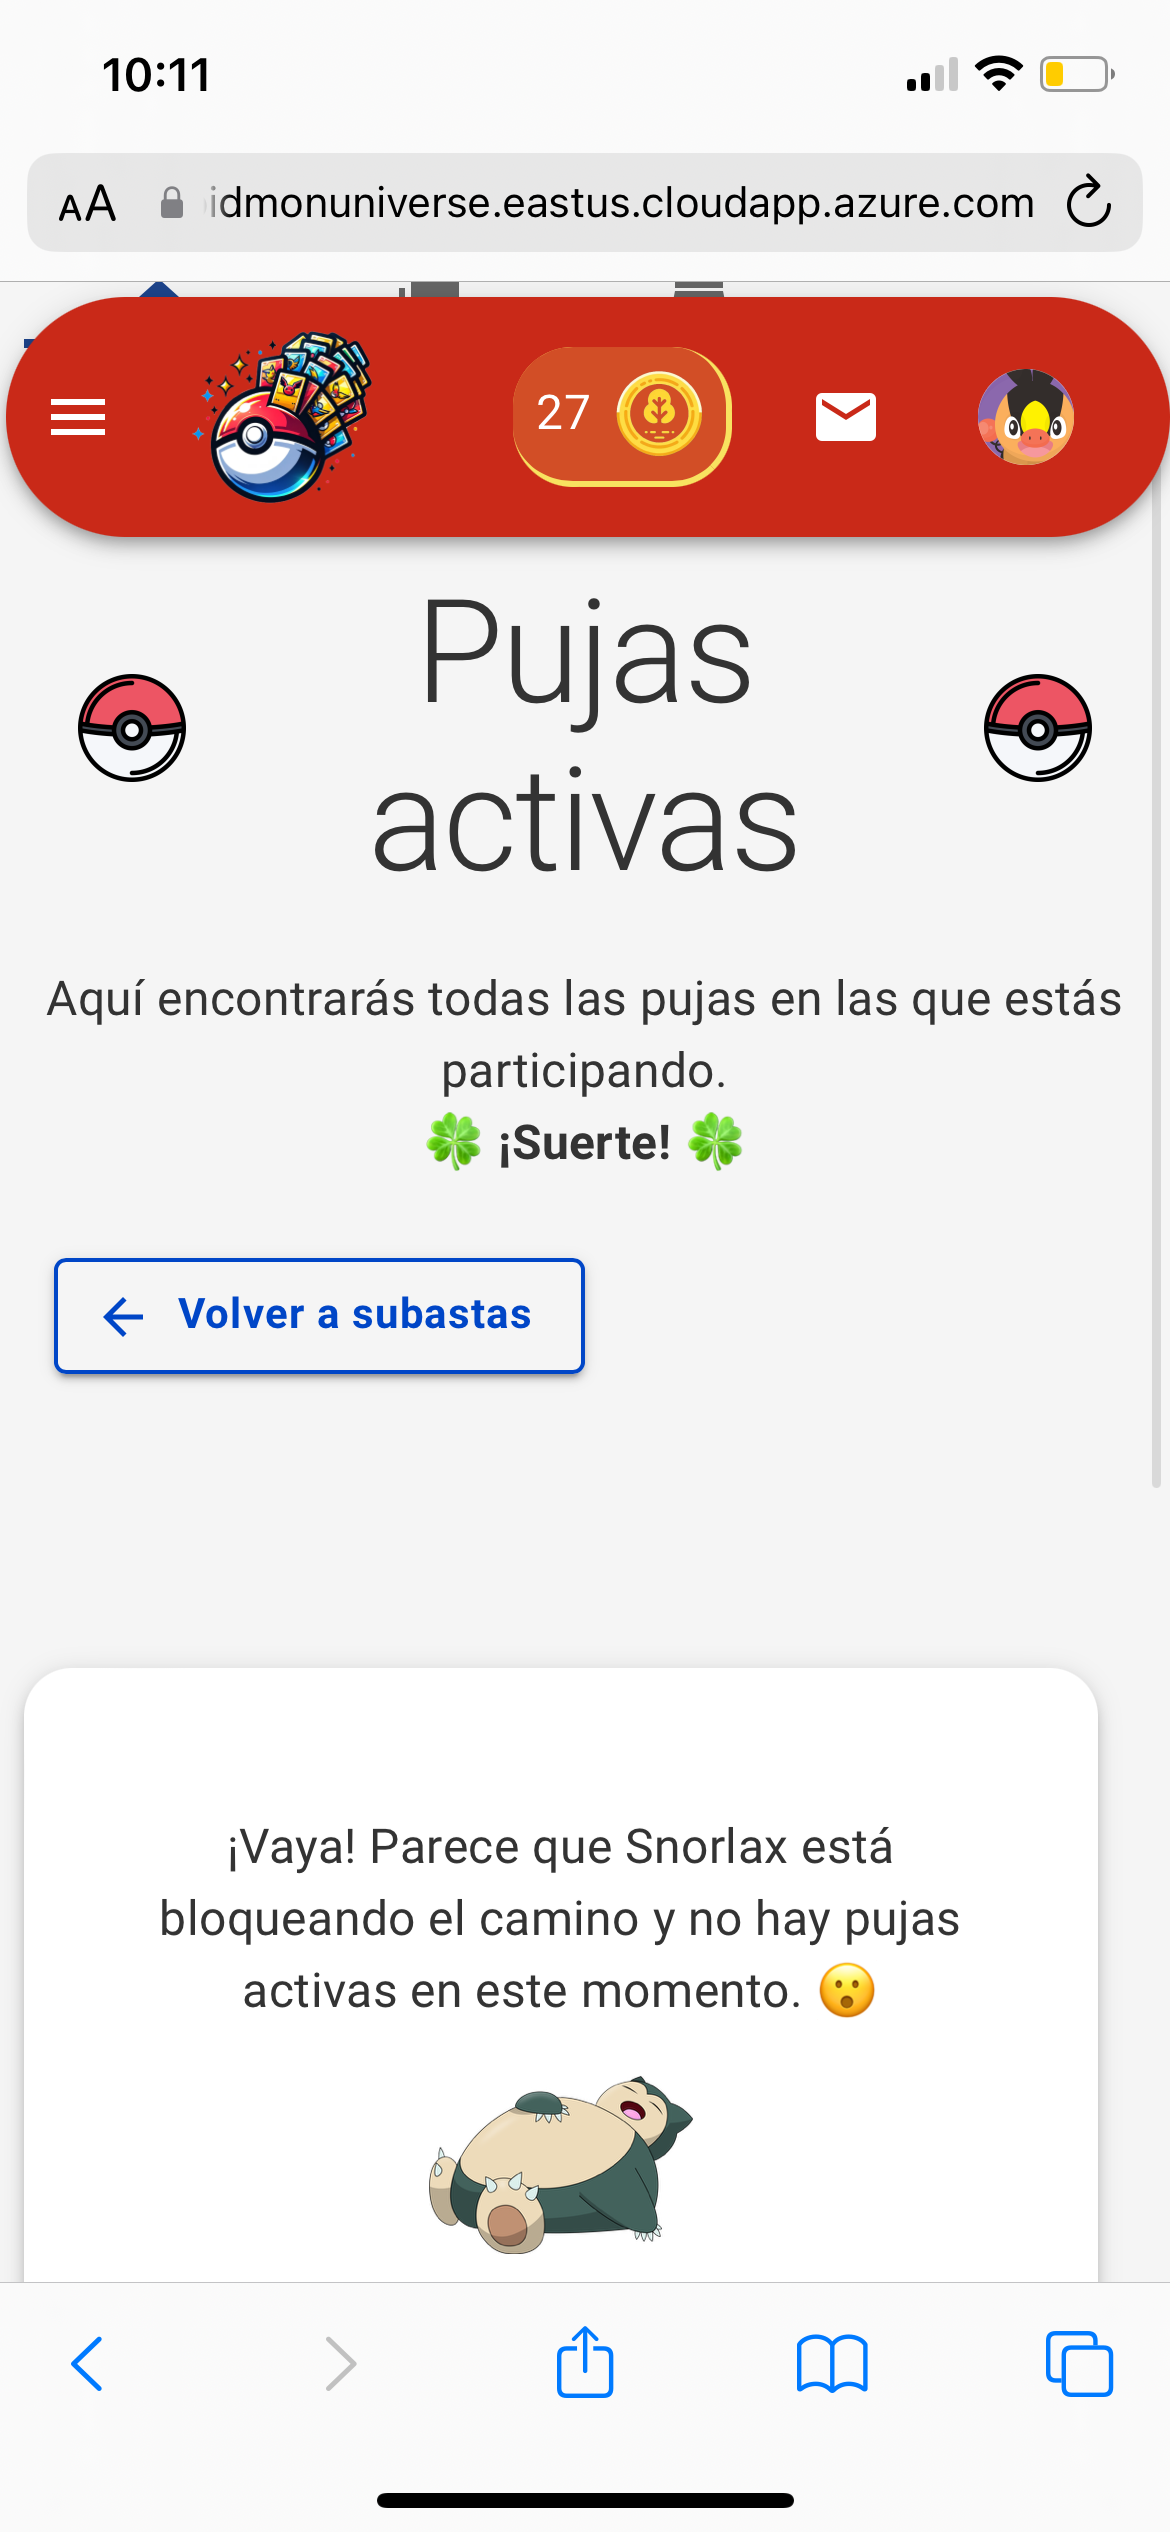
\includegraphics[width=0.2\textwidth]{figures/adaptabilidad/pujas.png}
    \caption{Adaptabilidad Página Mis pujas activas}
    \label{fig:Adap-Mis-Pujas}
\end{figure}

\subsection*{Recarga de saldo}
\begin{figure}[H]
    \centering
    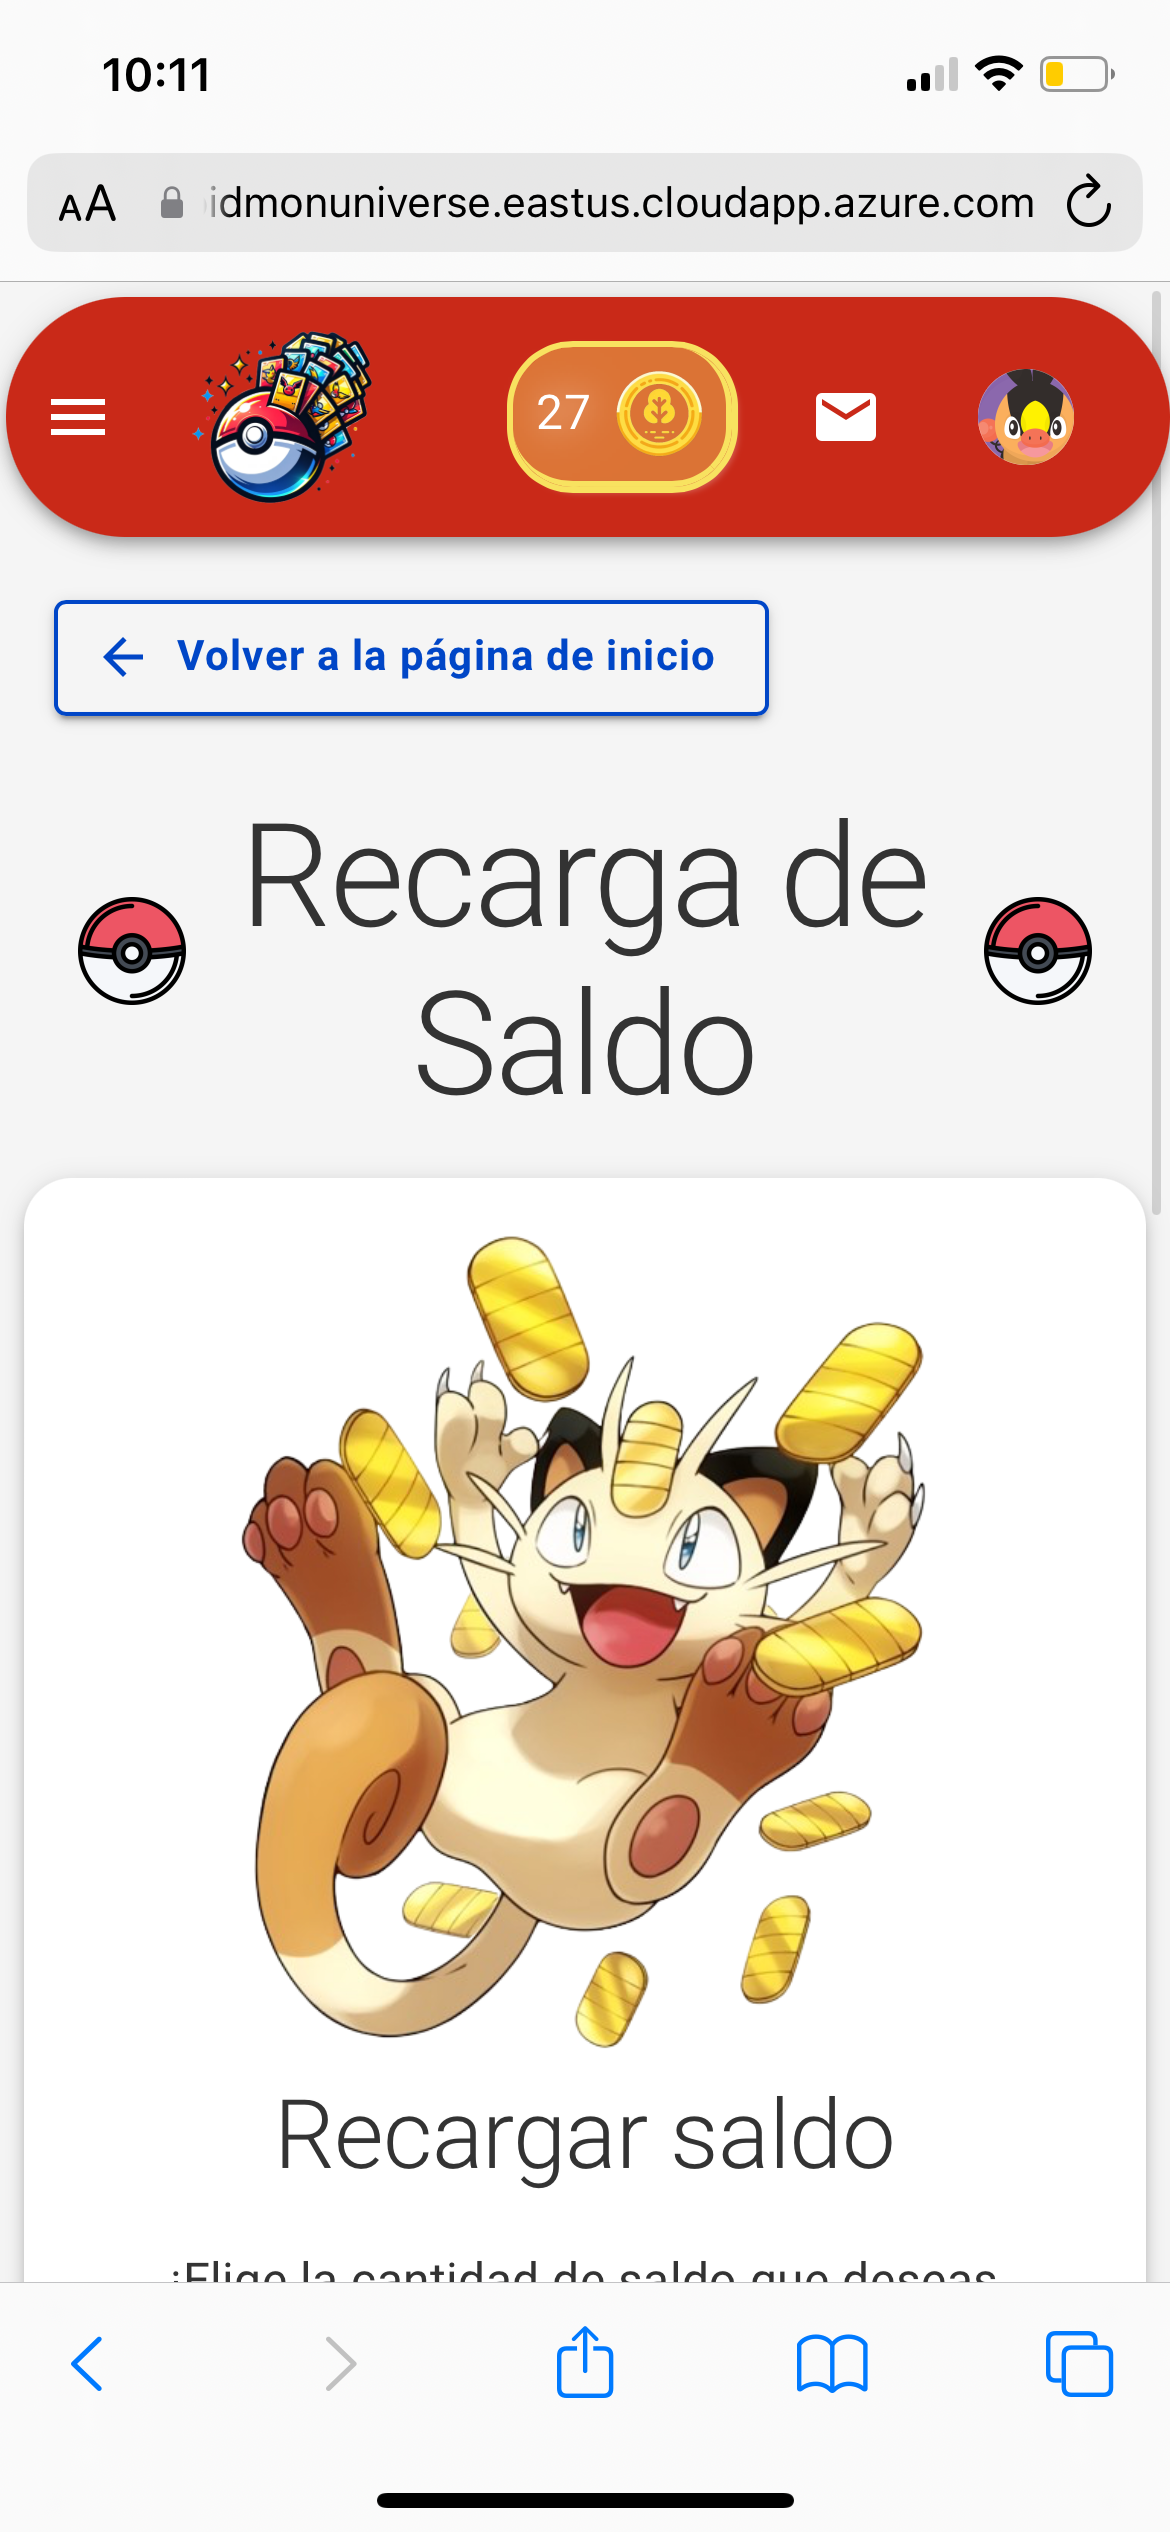
\includegraphics[width=0.2\textwidth]{figures/adaptabilidad/recarga.png}
    \caption{Adaptabilidad Página Recarga de saldo}
    \label{fig:Adap-Recarga}
\end{figure}

\subsection*{Historial de transacciones}
En la versión móvil se puede hacer clic en una celda de la tabla para ver los detalles de la transacción.
\begin{figure}[H]
    \centering
    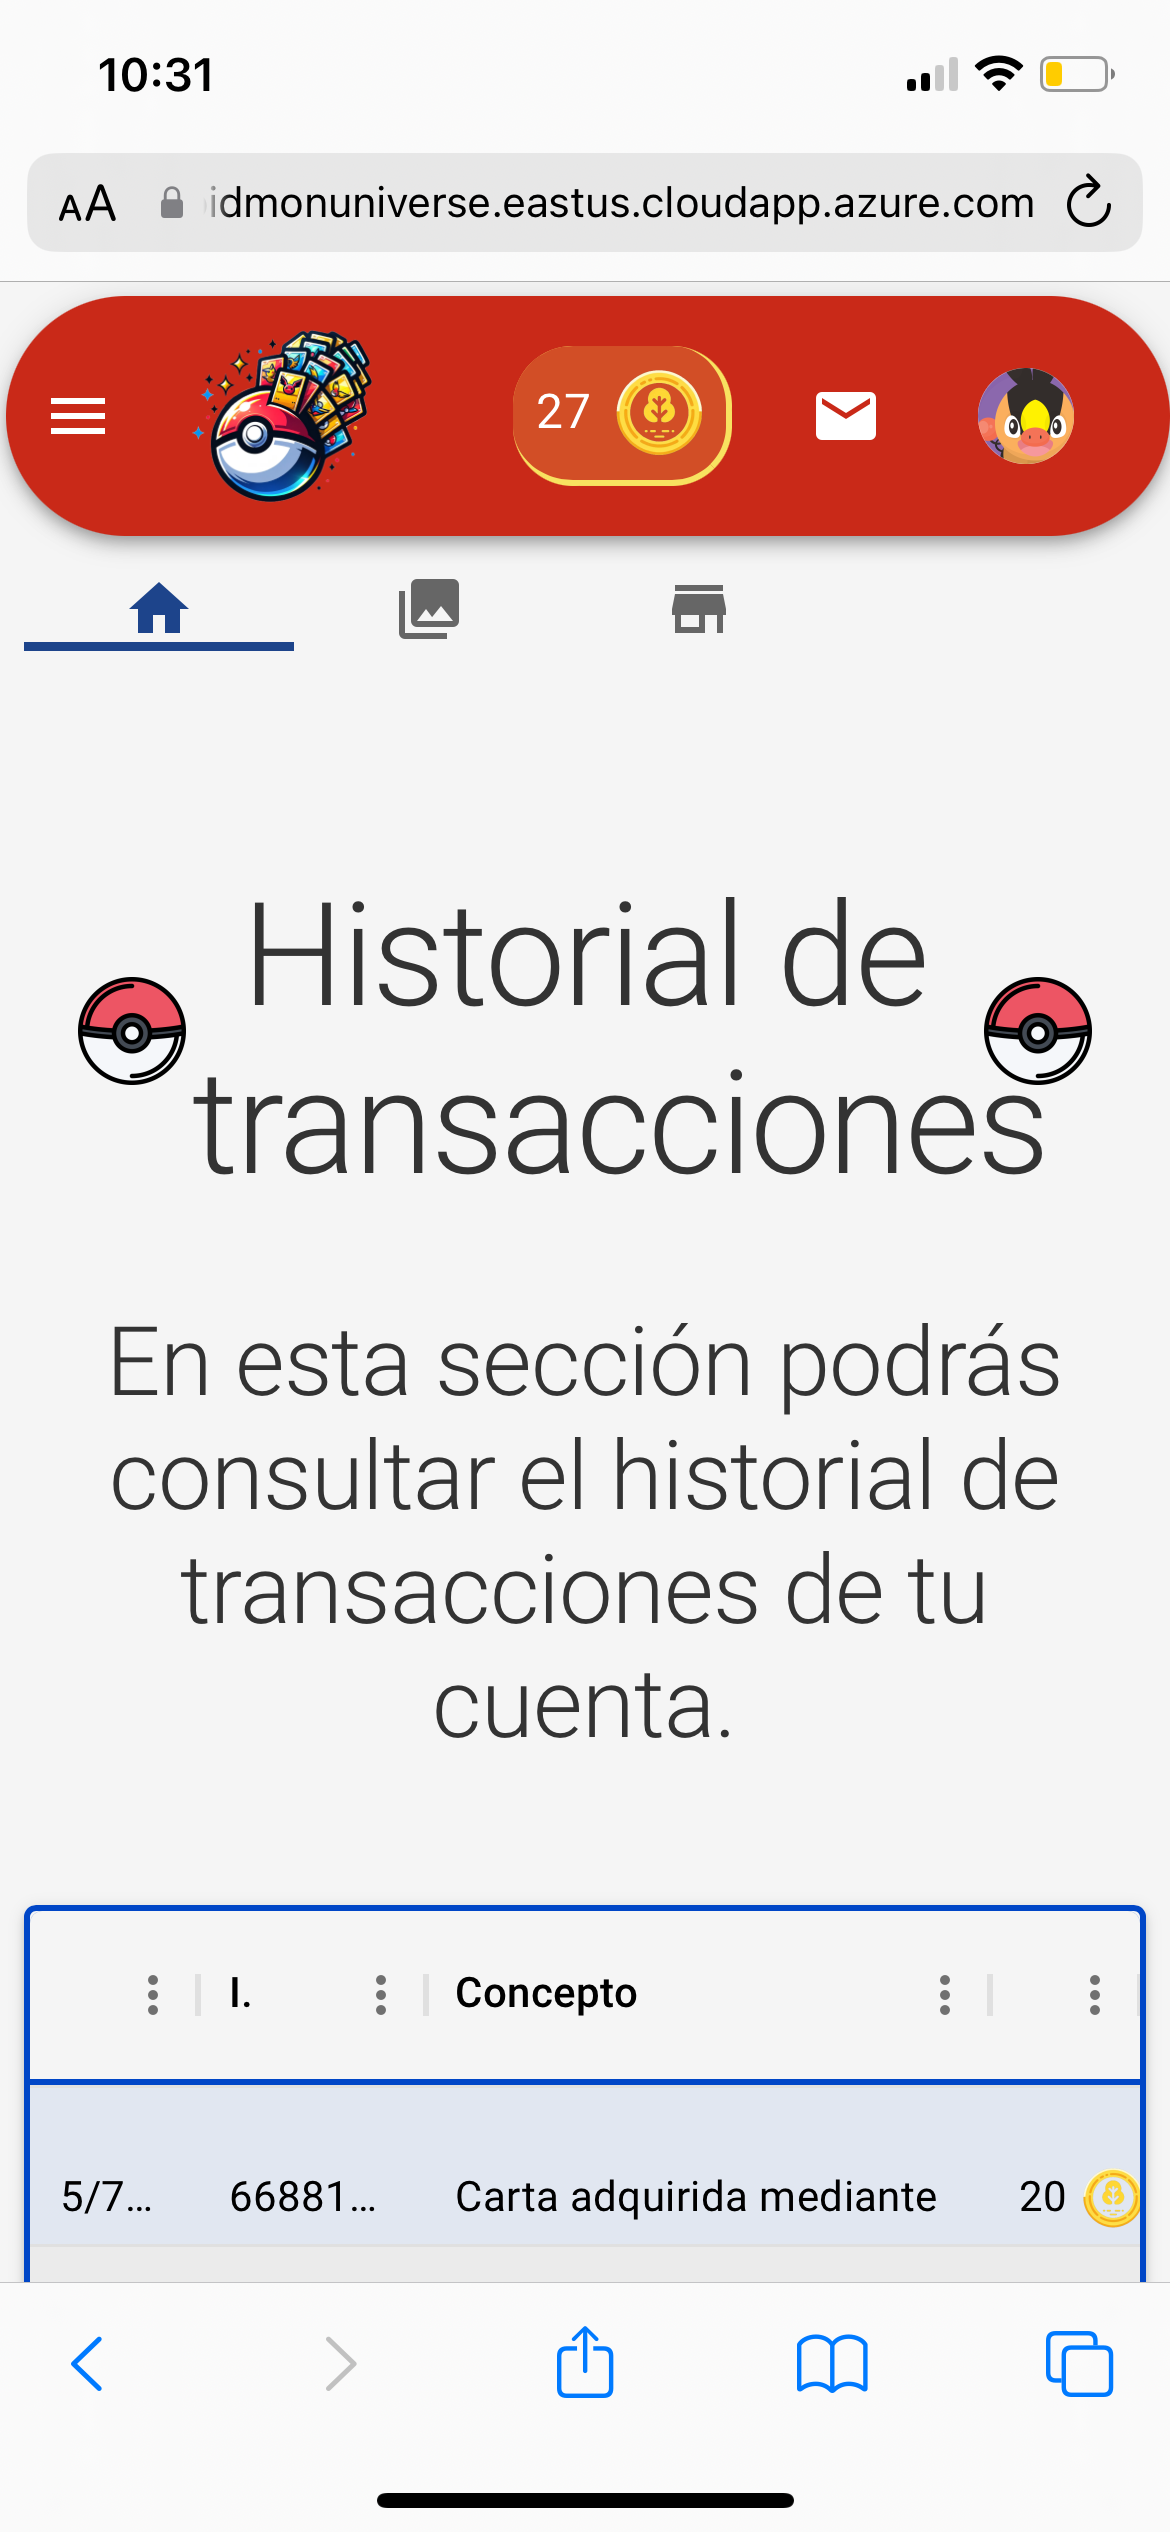
\includegraphics[width=0.2\textwidth]{figures/adaptabilidad/transacciones_1.png}
    \caption{Adaptabilidad Página Historial de transacciones}
    \label{fig:Adap-Historial}
\end{figure}

\begin{figure}[H]
    \centering
    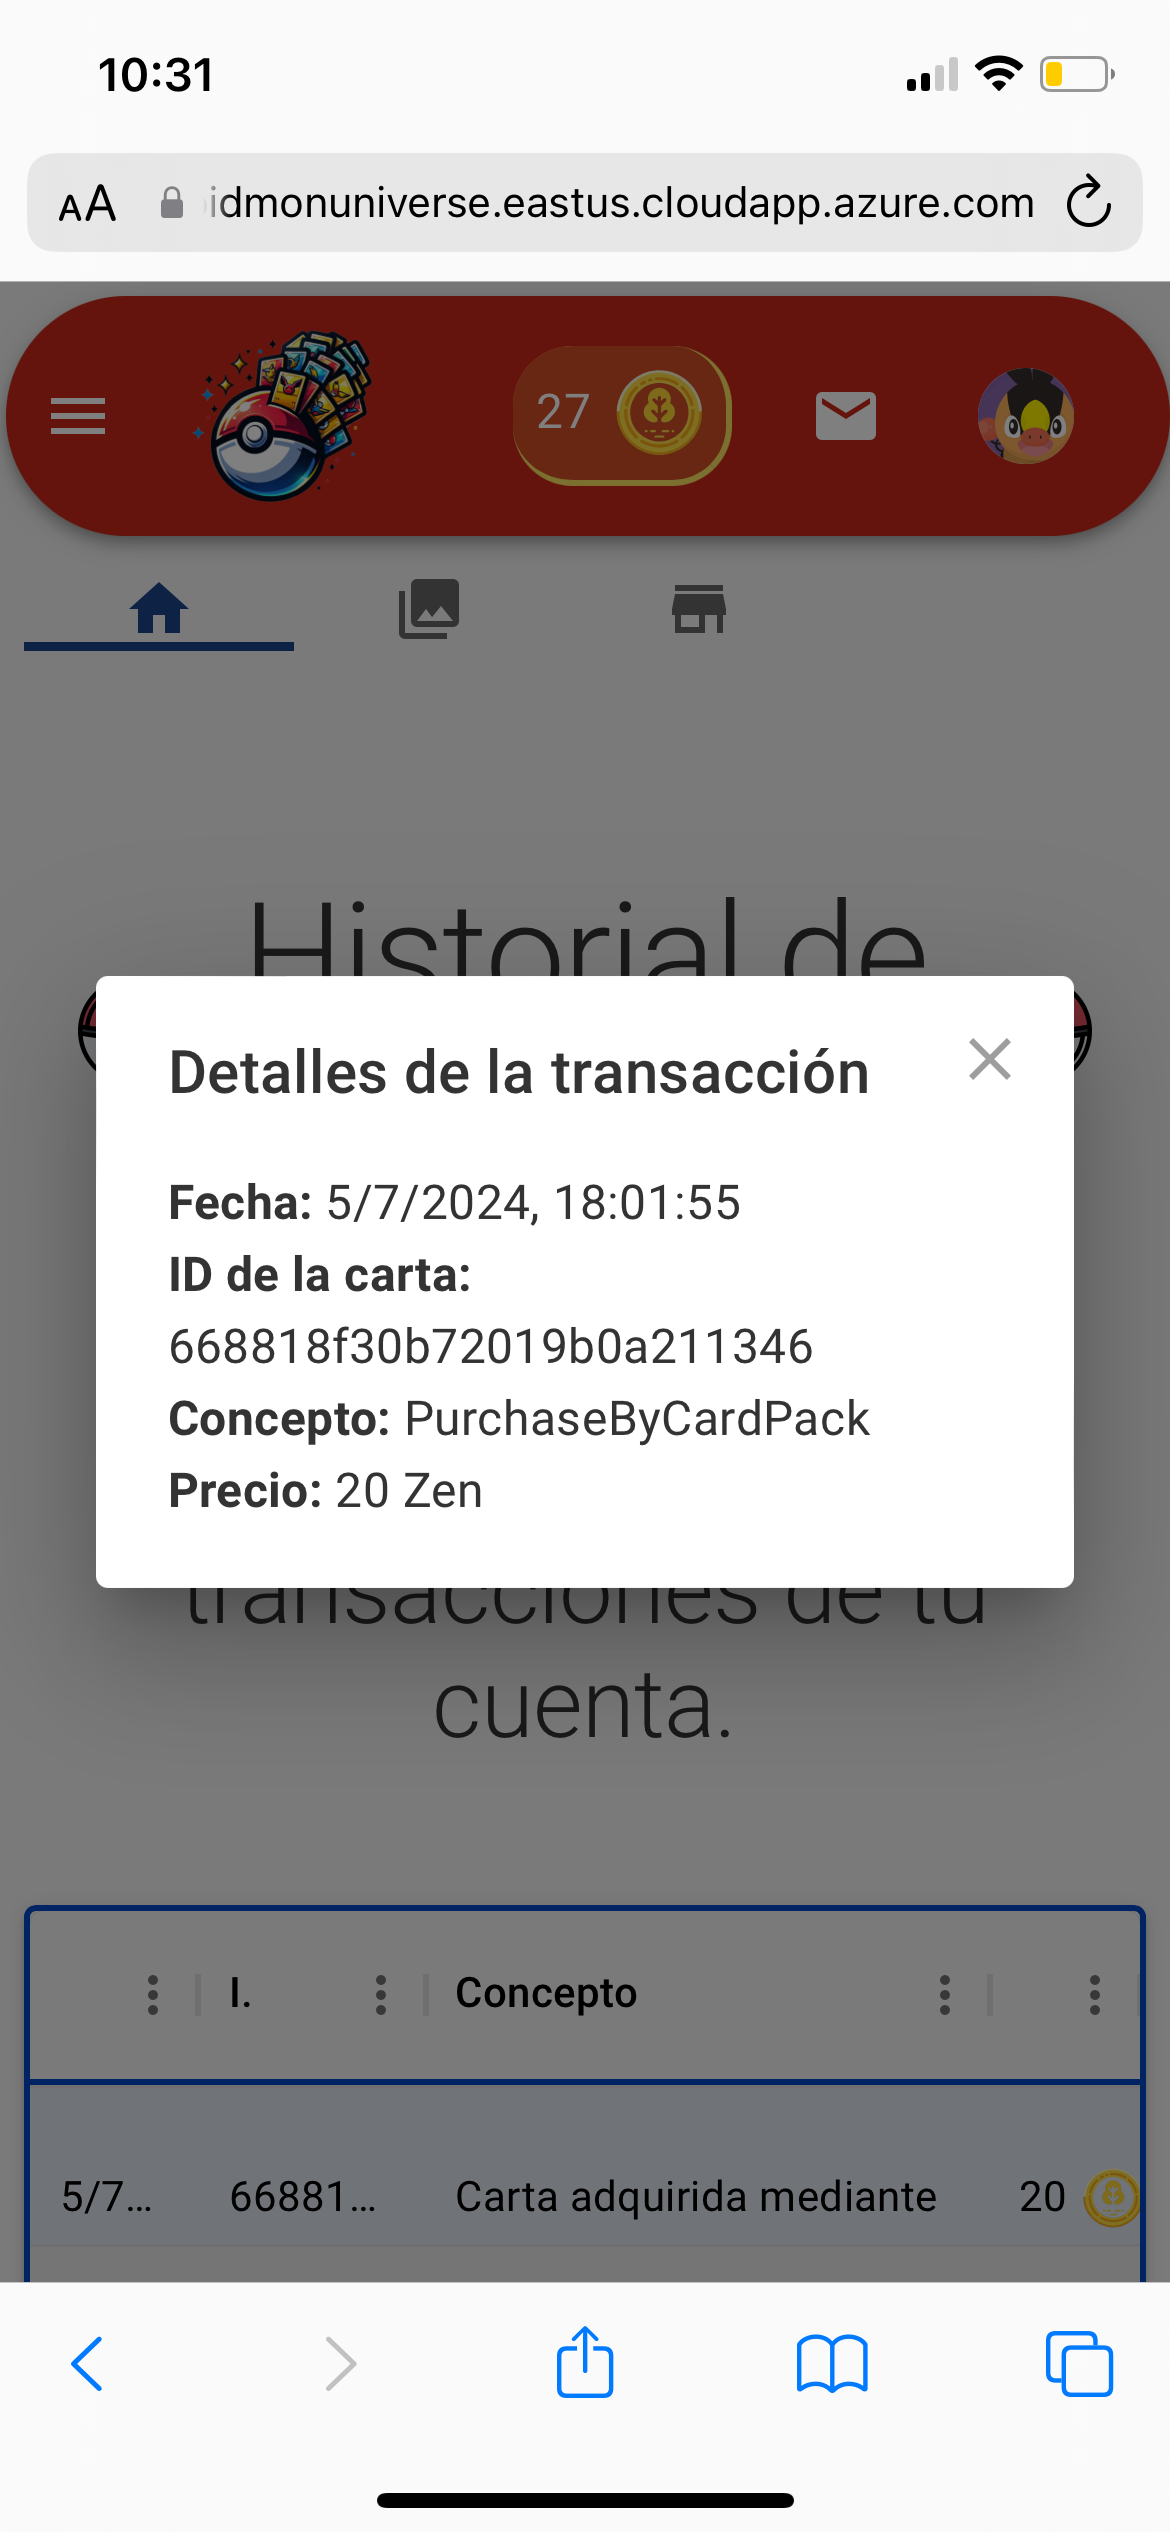
\includegraphics[width=0.2\textwidth]{figures/adaptabilidad/transacciones_2.png}
    \caption{Adaptabilidad Detalle de una transacción}
    \label{fig:Adap-Detalle-Transaccion}
\end{figure}


\subsection*{Actualizar perfil}
\begin{figure}[H]
    \centering
    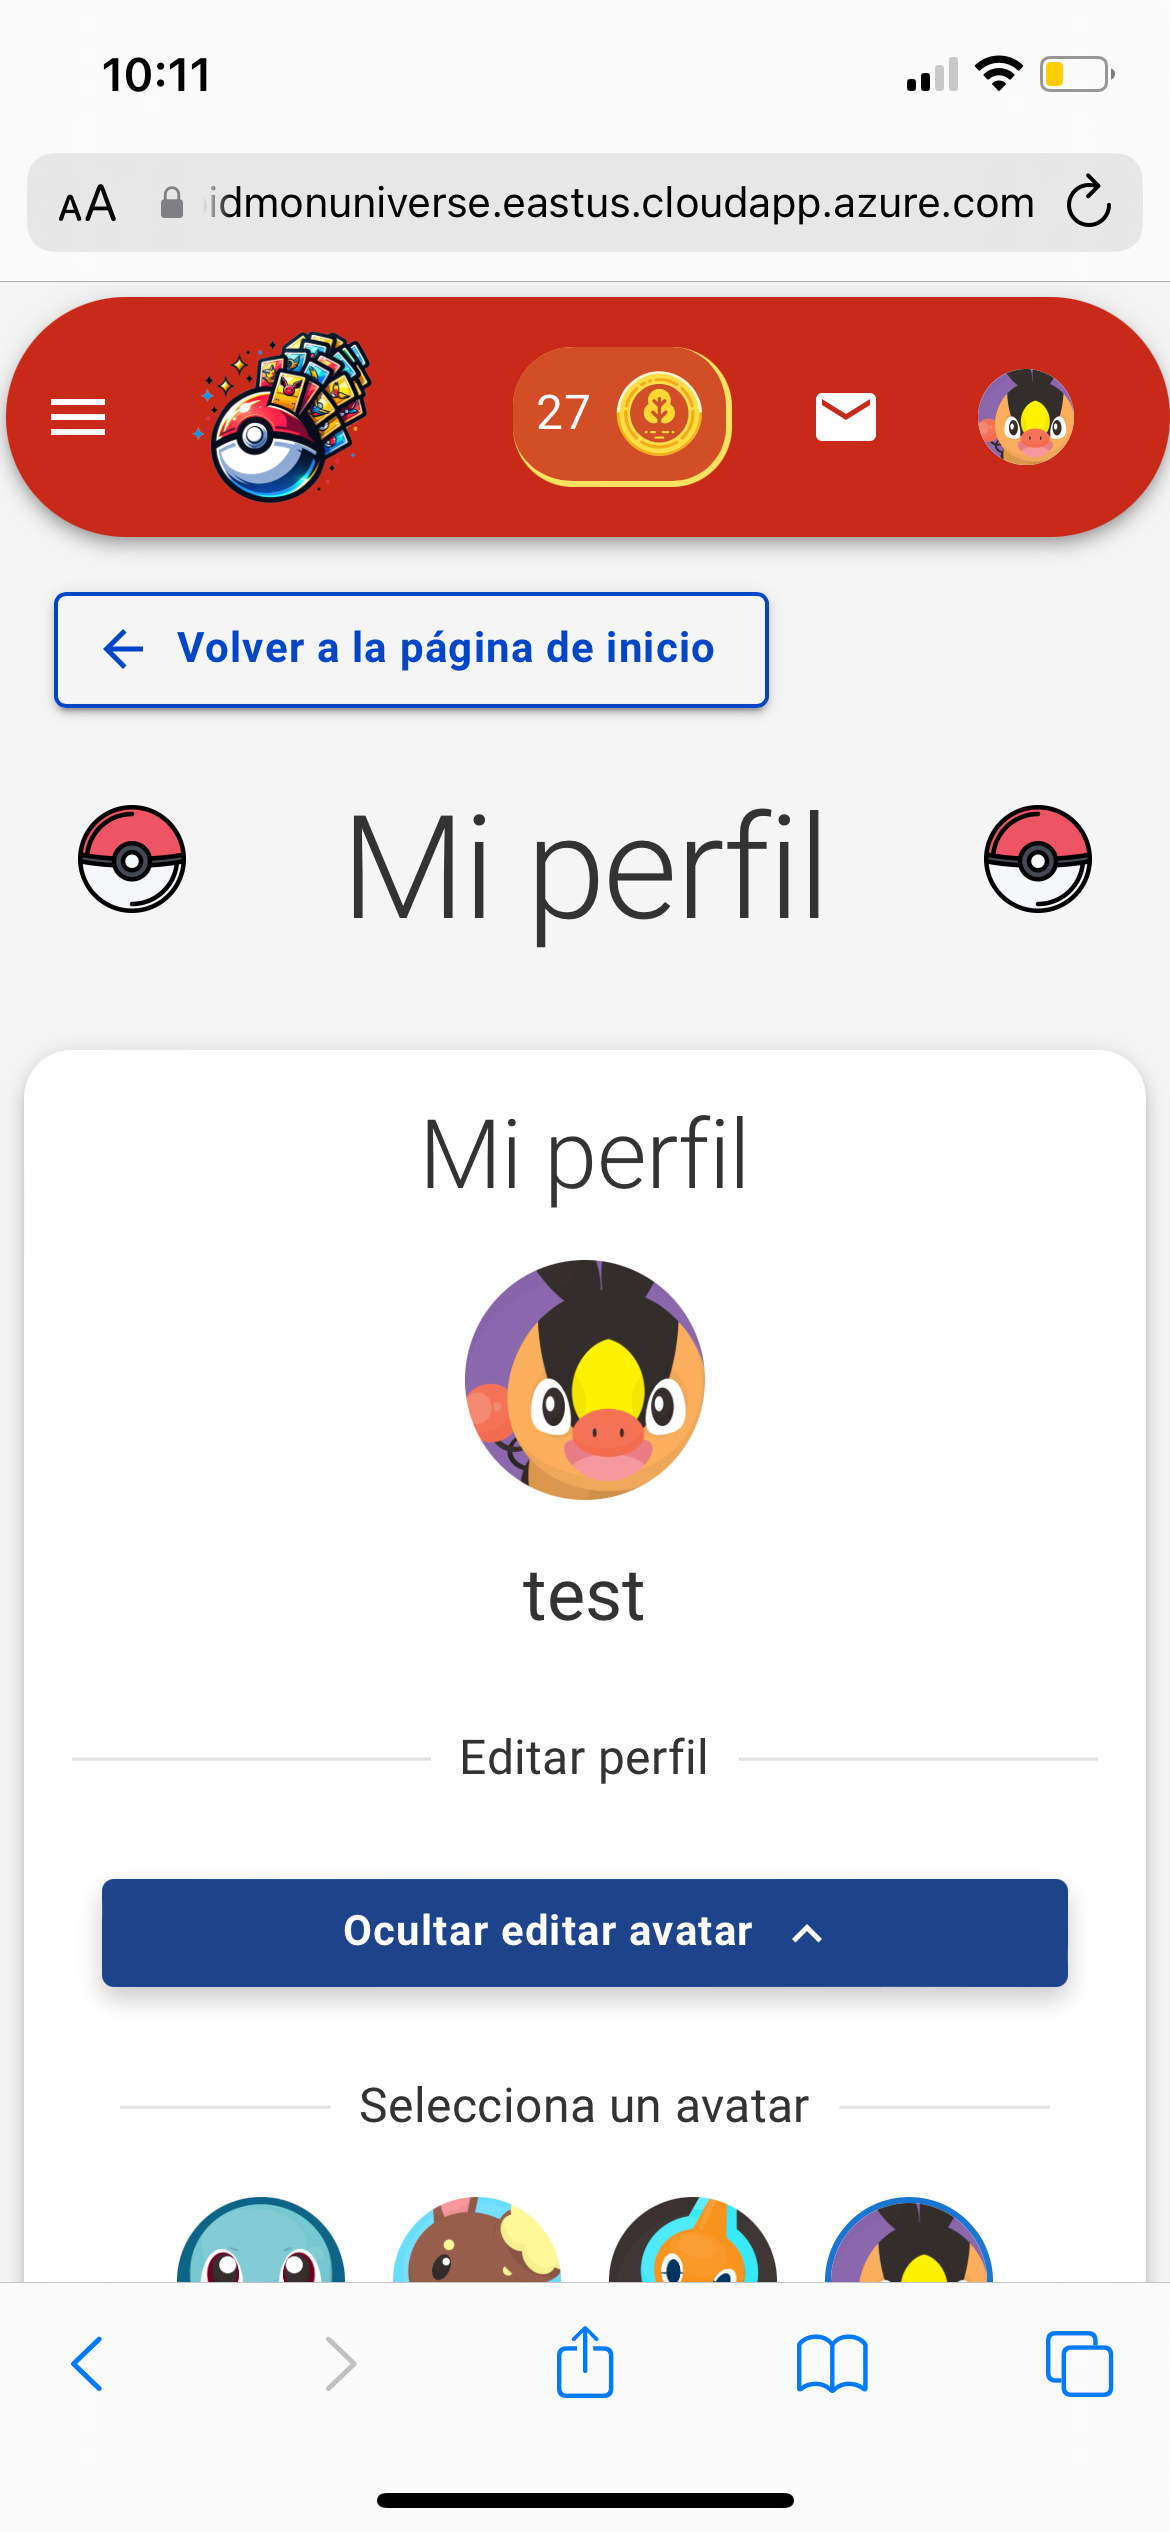
\includegraphics[width=0.2\textwidth]{figures/adaptabilidad/perfil.png}
    \caption{Adaptabilidad Página Actualizar perfil}
    \label{fig:Adap-Actualizar-Perfil}
\end{figure}


\subsection*{Menú general de la aplicación (usuario autenticado)}
\begin{figure}[H]
    \centering
    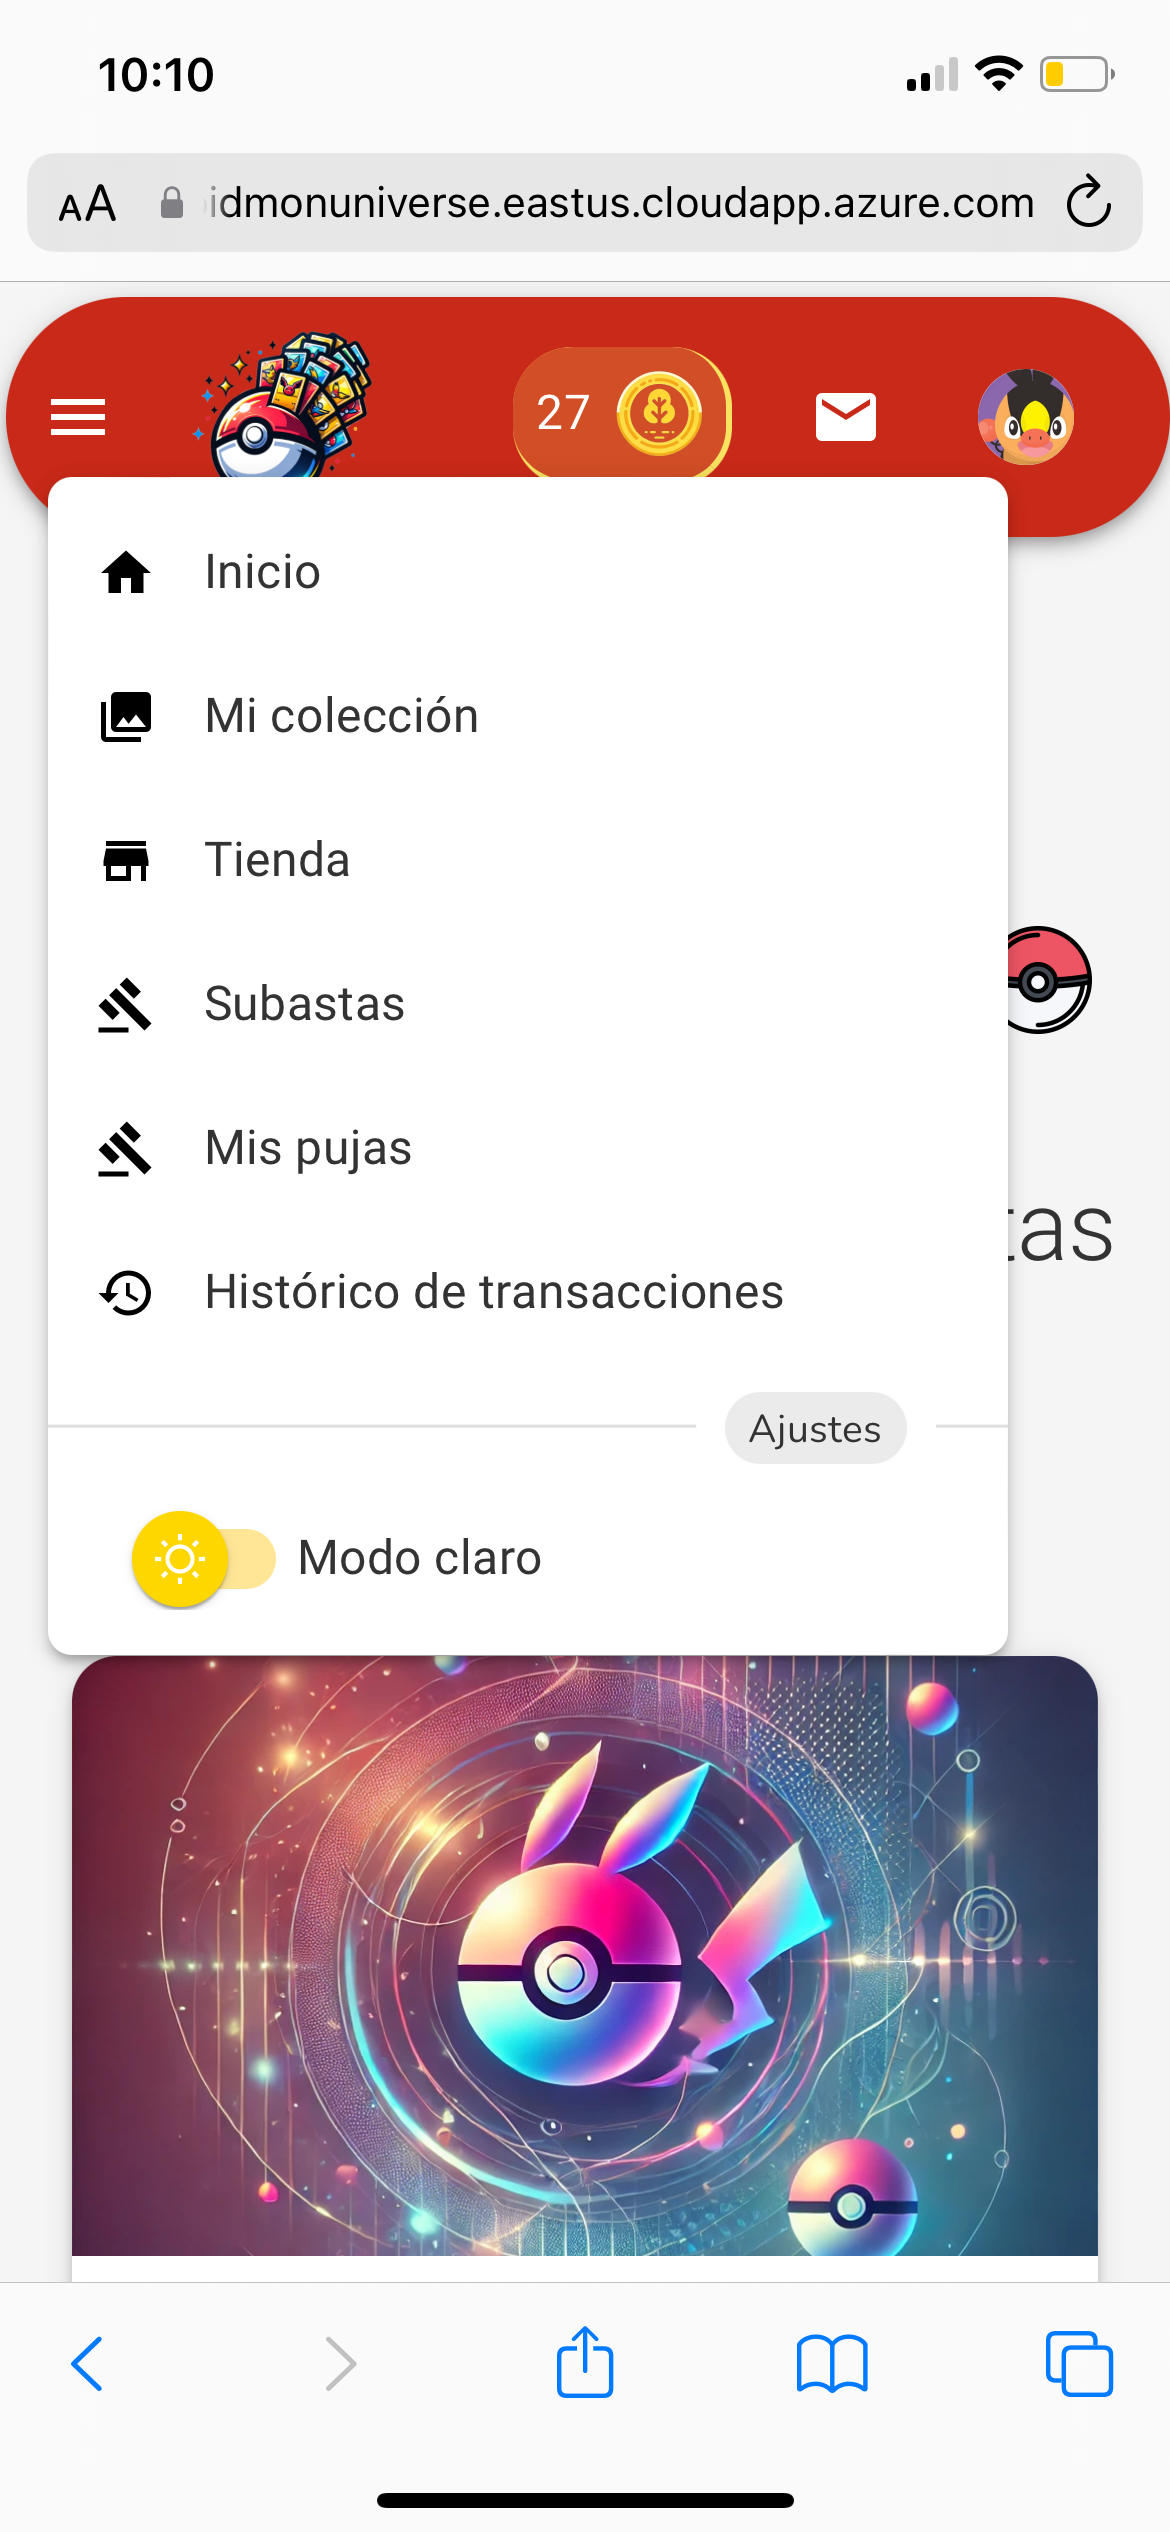
\includegraphics[width=0.2\textwidth]{figures/adaptabilidad/menu.png}
    \caption{Adaptabilidad Menú general de la aplicación}
    \label{fig:Adap-Menu}
\end{figure}


\subsection*{Resumen de los resultados}
La aplicación cumple con los requisitos de adaptabilidad a diferentes resoluciones de pantalla.
Se ha comprobado la adaptabilidad de la aplicación en las resoluciones de pantalla más comunes, como las de los dispositivos móviles, tablets y portátiles.